% arara: PDFLaTeX
% arara: nomencl
% arara: PDFLaTeX
\documentclass[a4paper,12pt]{report}
\usepackage[utf8]{vietnam}
\usepackage{amsmath}
\usepackage{amsfonts}
\usepackage{comment}
%\usepackage{enumitem}
\usepackage{enumerate}
%\usepackage{amssymb}
\usepackage{graphicx}
%\usepackage{cases}
\usepackage{fancybox}
\usepackage{multirow}
\usepackage{longtable,booktabs}
\usepackage{listings}
\usepackage[nottoc]{tocbibind}
\usepackage{indentfirst}
\usepackage[english]{babel}
\usepackage{algpseudocode}
%\usepackage[refpage]{nomencl}

%\makenomenclature
\usepackage{acro}
\acsetup{
  only-used = false,
  list-style = extra-tabular
}

\usepackage{algorithm}
\usepackage{float}
\usepackage{tikz}
\usepackage{pgfplots}

\usepackage{tikz-uml}
\usetikzlibrary{arrows.meta}
\PassOptionsToPackage{hyphens}{url}\usepackage{hyperref}  
\usepackage[left=3cm, right=2.00cm, top=2.00cm, bottom=2.00cm]{geometry}
%\lstset{
   %keywords={break,case,catch,continue,else,elseif,end,for,function,
   %   global,if,otherwise,persistent,return,switch,try,while},
%   language = Java,
%   basicstyle=\ttfamily \fontsize{12}{15}\selectfont,   
	% numbers=left,
%   frame=lrtb,
%tabsize=3
%}
\hypersetup{
    colorlinks,
    citecolor=black,
    filecolor=black,
    linkcolor=blue,
    urlcolor=red 
}
\setlength{\parskip}{0.6em}
\addto\captionsenglish{%
 \renewcommand\chaptername{Chương}
 \renewcommand{\contentsname}{Mục lục} 
 \renewcommand{\listtablename}{Danh sách bảng}
 \renewcommand{\listfigurename}{Danh sách hình vẽ}
 \renewcommand{\tablename}{Bảng}
 \renewcommand{\figurename}{Hình}
 \renewcommand{\bibname}{Tài liệu tham khảo}
}

\makeatletter
\newcommand{\vast}{\bBigg@{4}}
\newcommand{\Vast}{\bBigg@{5}}
\newcommand{\vastl}{\mathopen\vast}
\newcommand{\vastm}{\mathrel\vast}
\newcommand{\vastr}{\mathclose\vast}
\newcommand{\Vastl}{\mathopen\Vast}
\newcommand{\Vastm}{\mathrel\Vast}
\newcommand{\Vastr}{\mathclose\Vast}
\makeatother

\algnewcommand\algorithmicforeach{\textbf{for each}}
\algdef{S}[FOR]{ForEach}[1]{\algorithmicforeach\ #1\ \algorithmicdo}
\newtheorem{definition}{Định nghĩa}[chapter]
%\newtheorem{lema}{Bổ đề}[chapter]
%\newtheorem{theorem}{Định lý}[chapter]
%Bang chu viet tắt---------------
\DeclareAcronym{ERP}{
  short = ERP ,
  long  = Enterprise Resource Planning ,
  class = abbrev
}
\DeclareAcronym{JSP}{
  short = JSP ,
  long  = Java Server Pages ,
  class = abbrev
}
\DeclareAcronym{FTL}{
  short = FTL ,
  long  = FreeMarker Template Language ,
  class = abbrev
}
\DeclareAcronym{SOAP}{
  short = SOAP ,
  long  = simple object access protocol là một dạng web service ,
  class = abbrev
}
\DeclareAcronym{GRASP}{
  short = GRASP ,
  long  = A Greedy Randomized Adaptive Search Procedure,
  class = abbrev
}
\DeclareAcronym{TSP}{
  short = TSP ,
  long  = Traveling salesman problem,
  class = abbrev
}
\DeclareAcronym{TSPD}{
  short = TSPD ,
  long  = Traveling salesman problem with Drone,
  class = abbrev
}
\DeclareAcronym{CSP}{
  short = CSP ,
  long  = bài toán thỏa mãn ràng buộc - Constraint Satisfaction Problem ,
  class = abbrev
}
\DeclareAcronym{DD}{
  short = DD ,
  long  = một chuyến giao hàng bởi drone - drone delivery ,
  class = abbrev
}

\DeclareAcronym{TD}{
  short = TD ,
  long  = một hành trình giao hàng bởi xe tải - truck delivery,
  class = abbrev
}
% class `nomencl': nomenclature

%--------------------------------
\begin{document}
\thispagestyle{empty}
\thisfancypage{
\setlength{\fboxrule}{1pt}
\doublebox}{}

\begin{center}
{\fontsize{16}{19}\fontfamily{cmr}\selectfont TRƯỜNG ĐẠI HỌC BÁCH KHOA HÀ NỘI\\
VIỆN CÔNG NGHỆ THÔNG TIN VÀ TRUYỀN THÔNG}\\
\textbf{------------*******---------------}\\[1cm]

\includegraphics[scale=0.13]{hust.jpg}\\[1.3cm]
{\fontsize{23}{43}\fontfamily{cmr}\selectfont ĐỒ ÁN TỐT NGHIỆP}\\[0.1cm]
{\fontsize{25}{10}\fontfamily{cmr}\fontseries{b}\selectfont NGÀNH KHOA HỌC MÁY TÍNH}\\[0.9cm]
{\fontsize{20}{24}\fontfamily{phv}\selectfont Phát triển thuật toán tìm kiếm cục bộ cho bài toán lập lộ trình giao hàng kết hợp xe tải và thiết bị bay drone}\\[2cm]

\hspace{-5cm}\fontsize{14}{16}\fontfamily{cmr}\selectfont \textbf{Sinh viên thực hiện:}\\[0.1cm] 
\begin{longtable}{l c c}
Nguyễn Tuấn Đạt & 20130856 & CNTT2.02-K58 
\end{longtable}
\vspace{0.3cm}
\hspace{-8.5cm}\fontsize{14}{16}\fontfamily{cmr}\selectfont \textbf{Giảng viên:}\\[0.1cm]
\hspace{-2.7cm}\fontsize{14}{16}\fontfamily{cmr}\selectfont TS. Phạm Quang Dũng \\[3cm]
\fontsize{16}{19}\fontfamily{cmr}\selectfont Hà Nội 12--2017
\end{center}
\addcontentsline{toc}{chapter}{Lời cảm ơn}
\chapter*{Lời cảm ơn}
Trước khi trình bày nội dung của đồ án này, tôi xin được gửi lời cảm ơn sâu sắc và chân thành nhất đến TS. Phạm Quang Dũng, người đã tận tình hướng đẫn tôi trong suốt quá trình thực hiện đồ án này cũng như những năm tháng học tại trường Đại học Bách Khoa Hà Nội. Đồng thời tôi cũng xin bày tỏ lòng biết ơn đến các thầy cô trường Đại học Bách Khoa Hà Nội, Viện công nghệ thông tin và truyền thông, đặc biệt là các thầy cô bộ môn Khoa học máy tính đã tận tình chỉ dạy cho tôi trong những năm tháng học tập ở trường. \\ 

Tôi cũng xin bày tỏ lòng biết ơn đến các anh chị ở công ty cổ phần OLBIUS đã nhiệt tình giúp đỡ tôi phần công nghệ cho đồ án này. Cùng với đó, tôi cũng xin cảm ơn các anh chị ở lab MSO đã giúp đỡ tôi trong những năm tháng tôi sinh hoạt ở lab.\\

Cuối cùng tôi xin gửi lời cảm ơn đến gia đình, bạn bè đã luôn ở bên tôi, đông viên và giúp đỡ tôi trong suốt quá trình học tập và thực hiện đồ án tốt nghiệp. 
\newpage
\pdfbookmark{\contentsname}{toc}

\tableofcontents
\newpage
\chapter*{Bảng chữ viết tắt}
\printacronyms[include-classes=abbrev,heading=none]

%\printacronyms[include-classes=nomencl,name=Danh mục]
%\listoftables
\listoffigures


%\printnomenclature
\addcontentsline{toc}{chapter}{Mở đầu}
\chapter*{Giới thiệu chung}
Bài toán lập lịch vận chuyển hàng hóa từ lâu đã là lớp bài toán tối ưu hóa quan trọng và có tính thực tiễn cao. Công nghệ ngày càng phát triển, đặc biệt gần đây, phương tiện bay không người lái trở phổ biến với nhiều mẫu mã đặc trưng cho các mục đích sử dụng khác nhau. Thiết bị bay không người lái (hay còn gọi là drone) đã và đang được nghiên cứu sử dụng trong ngành công nghiệp vận chuyển hàng hóa. Với công nghệ hiện nay, drone có thể nâng những vật có khối lượng hàng chục kilogram và quãng đường bay có thể đạt đến hàng chục kilometers. Những đặc tính trên khiến thiết bị bay không người lái có thể là xu hướng trong nhiều năm tới đây.

Trong thời buổi công nghệ thông tin phát triển rộng khắp như hiện nay. Bài toán lập lịch vận chuyển hàng hóa gần như là một phần không thể thiếu trong hệ thống \ac{ERP} (Enterprise Resource Planning) của các công ti vận tải hàng đầu thế giới. Chính vì vậy trong đồ án này, chúng tôi đã phát triển và cài đặt mô hình thuật toán tìm kiếm cục bộ cho bài toán lập lộ trình giao hàng kết hợp xe tải và thiết bị bay không người lái ứng dụng vào công nghệ Ofbiz dưới dạng web service. Ofbiz là một ứng dụng mã nguồn mở về \ac{ERP} được Apache phát triển từ năm 2001. Ofbiz cho phép lập trình viện có thể can thiệp, thay đổi hệ thống linh hoạt cũng như có khả năng phát triển một ứng dụng độc lập hoàn chỉnh. 

Nội dung chính của đồ án bao gồm 6 chương:
\begin{itemize}
\item \textbf{Chương 1:} Cơ sở lý thuyết
\item \textbf{Chương 2:} Bài toán lập lộ trình giao hàng kết hợp một xe tải với một thiết bị bay cùng các nghiên cứu liên quan.
\item \textbf{Chương 3:} Đề xuất thuật toán tìm kiếm cục bộ giải bài toán lập lộ trình vận tải giao hàng kết hợp một xe tải và nhiều thiết bị bay.
\item \textbf{Chương 4:} Kết quả thử nghiệm.
\item \textbf{Chương 5:} Thiết kế chương trình ứng dụng.
\item \textbf{Chương 6:} Kết luận và hướng phát  triển.
\end{itemize}

\chapter{Cơ sở lý thuyết}
Trong chương này chúng tôi sẽ trình bày cơ sở lý thuyết chung cho bài toán tối ưu hóa tổ hợp, tối ưu hóa thỏa mãn ràng buộc. Các định nghĩa bài toán tối ưu hóa tổ hợp, bài toán thỏa mãn ràng buộc và ứng dụng được trình bày trong phần \ref{section:cbo}. Ở phần \ref{section:cbs} chúng tôi trình bày hai hướng tiếp cận giải bài toán thỏa mãn ràng buộc là thuật toán giải đúng và thuật toán giải gần đúng. Trong phần \ref{section:ofbiz}, chúng tôi giới thiệu tổng quan về công nghệ chính xây dựng module ứng dụng cho đồ án này là công nghệ Ofbiz. Các tài liệu tham khảo chúng tôi sử dụng trong phần này là \cite{TRR}\cite{AIAMAB}\cite{slidethayquang}\cite{csplib30} \cite{TUHTT}\cite{CBLS}\cite{DAA}\cite{HCP}\cite{GA}\cite{AOW}.
\section{Tối ưu hóa tổ hợp và ứng dụng}
\label{section:cbo}
\subsection{Tối ưu hóa tổ hợp}
Bài toán tối ưu hóa tổ hợp dưới dạng tổng quát có thể được phát biểu như sau: \\

Tìm cực tiểu hay cực đại của phiến hàm $$f(x)\rightarrow min(max), x \in D$$ trong đó $D$ là một tập hữu hạn các phần tử. Hàm $f(x)$ được gọi là hàm mục tiêu của bài toán. Mỗi phần tử $x\in D$ được gọi là một phương án của bài toán, tập $D$ gọi là tập các phương án của bài toán. Phương án $x^* \in D$ đem lại giá trị nhỏ nhất (lớn nhất) cho hàm được gọi là phương án tối ưu, khi đó $f^*=f(x^*)$ được gọi là giá trị tối ưu của bài toán\cite{TRR}.
\subsubsection{Bài toán thỏa mãn ràng buộc}
Một ràng buộc \cite{AIAMAB} \cite{slidethayquang} là một quan hệ trên trên một tập các biến. Mỗi biến có một tập hữu hạn các giá trị có thể nhận gọi là miền giá trị. Một ràng buộc có thể được biểu diễn bằng một biểu thức toán học hoặc một bảng liệt kê các giá trị phù hợp cho các biến. 
Một \ac{CSP} bao gồm : \begin{enumerate}
\item Một tập các \textbf{biến} X.
\item Miền giá trị (một tập hữu hạn các giá trị) cho mỗi biến D.
\item Một tập hữu hạn các ràng buộc C.
\end{enumerate}  
Một trạng thái của bài toán được định nghĩa bởi một phép gán các giá trị cho tất cả các biến. Một trạng thái được gọi là lời giải khi nó thỏa mãn tất cả các ràng buộc trong $C$. Một vài bài toán \ac{CSP} còn yêu cầu tối ưu một hoặc nhiểu hàm mục tiêu.  \\

Chúng tôi trình bày hai ví dụ điển hình cho bài toán thỏa mãn ràng buộc là bài toán N con hậu và bài toán cân bằng chương trình học.
\subsubsection{N con hậu (N-QUEEN)}
Bài toán yêu cầu xếp $n$ quân hậu trên bàn cờ vua $n\times n$ sao cho không có hai quân hậu bất kì nào ăn được nhau.

\paragraph{Mô hình toán học}
\subparagraph{Biến}
Gọi $X=\{x_i|i \in [1,n]\}$ với $x_i$ có giá trị là cột của con hậu hàng thứ i.
\subparagraph{Miền giá trị}
$x_i \in [1,n]$\\
 Vd:  $x_1=2$ sẽ tương ứng với con hậu hàng thứ nhất đang đứng ở cột thứ 2.
\subparagraph{Các ràng buộc}
\begin{itemize}
\item Các con hậu không được ở trên cùng một cột.
$$ \forall i \neq j,x_i \neq x_j,  \quad i,j \in [1,n] $$
\item Các con hậu không cùng trên một hàng chéo.
$$\forall i \neq j,x_i-x_j \neq i-j , \quad i,j \in [1,n]$$
$$\forall i \neq j,x_j-x_i \neq i-j, \quad i,j \in [1,n]$$
\end{itemize} 
\subsubsection{Cân bằng lịch học (Balanced Academic Curriculum Problem) }
Bài toán yêu cầu thiết kế một chương trình học, được định nghĩa bằng việc sắp xếp các lớp vào các kì học sao cho thỏa mãn các quy định và cân bằng cho mỗi kì. Một chương trình học phải thỏa mãn các quy định sau:
\begin{itemize}
\item Một chương trình học định nghĩa bởi một tập các lớp học và tập các mối quan hệ giữa chúng.
\item Số lượng kì: một chương trình học chỉ được phép kéo dài trong một số kì nhất định.
\item Định lượng: Mỗi lớp học có một chỉ số tín chỉ khi mà hoàn thành lớp mỗi sinh viên nhận được tích lũy.
\item Lớp tiên quyết: Có một số lớp cần có những lớp khác học trước.
\item Giới hạn tín chỉ: Trong một kì sinh viên không được học quá ít, hoặc quá nhiều tín chỉ.
\item Số lớp tối thiểu: Số lượng lớp tối thiểu trong một kì của sinh viên.
\item Số lớp tối đa: Số lượng lớp tối đa trong một kì của sinh viên.
\end{itemize}
Mục đích của vấn đề là xếp các lớp vào các kì sao cho thỏa mãn tất cả các quy định trên và  chênh lệch số lượng tín chỉ trong các kì là nhỏ nhất.\cite{csplib30}
\paragraph{Mô hình toán học}
\subparagraph{Đầu vào}
\begin{itemize}
	\item $nPeriods$ là số lượng kì cần xếp lịch.
	\item $nCourses$  là số lượng lớp cần xếp lịch.
	\item $prereq$ là một danh sách các phần tử có dạng $\langle i,j \rangle $ thể hiện lớp $i$ cần phải được học trước lớp $j$.
	\item $credit(j)$ là số lượng tín chỉ của lớp $j$.
\end{itemize}
\subparagraph{Biến}
Gọi $$X= \{ X_{ij}|i\epsilon [1,nPeriods],j\epsilon [1,nCourses]  \} $$

\subparagraph{Miền giá trị}
\begin{itemize}
\item $X_{i,j}=1$ nếu lớp j được đặt trong kì i
\item $X_{i,j}=0$ nếu ngược lại 
\end{itemize}
\subparagraph{Các ràng buộc}
Ta định nghĩa : $$load[i]=\sum_{j \in [1,nCourses] } credit(j) *X_{i,j}   ,\forall i \in [1,nPeriods]$$
\begin{itemize}
\item Một lớp tín chỉ trong một kì 
$$   \sum_{i \in [1,nPeriods] } X_{i,j}=1,\forall j \in[1,nCourses]  $$

\item Điều kiện học phần học trước $$ \forall\langle i,j\rangle \in prereq, \ \forall k \in [1,nPeriods]: k>1  $$
$$X_{k,j} \leq \sum^{k-1}_{r=1} X_{r,i} $$ 
\item Điều kiện giới hạn số tín chỉ trong một kì $$load[i] \leq b, \forall i \in [1,nPeriods]$$
\item Điều kiện giới hạn số lớp học trong một kì $$\forall i \in [1,nPeriods] | c \leq \sum_{j \in [1,nCourses]} X_{i,j} \leq d$$
\item Điều kiện cân bằng $$minium  C= (max_{i \in [1,nPeriods]} load[j] -min_{i \in [1,nPeriods]} load[j] $$
\end{itemize}
\subsection{Ứng dụng}
Trong phần này chúng tôi trình bày một vài bài toán tối ưu hóa tổ hợp cụ thể. Những bài toán này là những bài toán thực tiễn được phát biểu dưới dạng bài toán tối ưu hóa tổ hợp, qua đó thể hiện được bài toán tối ưu hóa tổ hợp có tính ứng dụng cao, đây cũng là động lực phát trển của lĩnh vực tối ưu hóa tổ hợp\cite{TUHTT}.
\subsubsection{Lập thời khóa biểu (SIE Course Timetabling)}



\paragraph{Đầu vào}
\begin{itemize}
\item Cho một tập ngày $D_1,\ldots, D_q$ mỗi ngày có $p$ tiết, vd: Thứ 2 có 6 tiết.
\item Cho một tập các giảng viên $P=\{P_1,\ldots,P_m\}$, mỗi giảng viên có một tập $B$ bao gồm các cặp $\langle \text{thứ},\text{tiết}\rangle$ mà giảng viên đó bận.
\item Một tập lớp sinh viên $CL=\{CL_1,\ldots,CL_k\}$
\item Một tập các lớp học môn học: $C=\{c_1,\ldots, c_n\}$ mỗi $c_i$ bao gồm 3 thông tin: 
	\begin{enumerate}
	\item $d(c_i)$ : số lượng tiết của lớp $c_i$
	\item $p(c_i)$ : giảng viên được yêu cầu dạy lớp $c_i$
	\item $cl(c_i)$ : tập các lớp sinh viên học trong $c_i$
	\end{enumerate}
\end{itemize} 
\paragraph{Đầu ra}
Xây dựng thời khóa biểu cho tập lớp $C$ trong tập ngày $D$.
\paragraph{Các ràng buộc}
\begin{itemize}
\item Hai lớp môn học bất kì có chung giảng viên thì không được trùng tiết trong một ngày.
\item Một buổi học không được trùng vào thời gian bận của giáo sư\cite{CBLS}.
\end{itemize}
\subsubsection{Phân công y tá}
\paragraph{Đầu vào}
Bài toán yêu cầu xếp lịch ca trực cho $n$ y tá trong $m$ ngày. Mỗi ngày có $k$ kíp trực khách nhau.  
\paragraph{Ràng buộc}
\subparagraph{Ràng buộc cứng}
\begin{itemize}
\item Mỗi y tá chỉ trực một ca trong ngày.
\item Mỗi y tá chỉ trực một số lượng thời gian nhất định.
\item Với một kíp số lượng lần trực của y tá không được vượt quá một đại lượng nhất định.
\item Mỗi y tá không có đợt nghỉ quá ngắn.***
\item Số lượng ca trực liên tục của một y tá không được quá nhiều hoặc quá ít.
\item Các y tá không được trực quá trong các đợt cuối tuần.***
\item Các y tá được đăng kí một số ngày họ được nghỉ.
\end{itemize}
\subparagraph{Ràng buộc mềm}
\begin{itemize}
\item Các y tá được phép yêu cầu nghỉ hoặc làm một số ca nào đó.
\item Bệnh viện yêu cầu số lượng y tá trong mỗi ca trực.
\end{itemize}

\subsubsection{Lập lộ trình vận tải}
Lớp bài toán lập lộ trình vận tải là một trọng những lớp bài toán tối ưu quan trọng trong ngành công nghiệp giao vận. Xét bài toán tổng quát được định nghĩa như sau:

Xét một mô hình vận tải gồm $m$ nhà cung ứng (hay còn gọi là điểm phát) và $n$ cửa hàng (điểm thu). Bài toán yêu cầu vận chuyển hàng hóa từ các  nhà cung ứng đến các cửa hàng sao cho chi phí di chuyển là nhỏ nhất.
\begin{itemize}
\item  $m$ nhà cung ứng.
\item  $n$ cửa hàng.
\item  $a_i$ lượng hàng nhà cung ứng $i$ cung cấp.
\item  $b_j$ lượng hàng cần nhập của cửa hàng $j$.
\item  $c_{ij}$ cước phí vận chuyển một đơn vị hàng từ nhà cung cấp $i$ đến cửa hàng $j$.\cite{TUHTT}
\end{itemize}
\begin {center}
\begin{tikzpicture}[
state/.style ={circle,draw}]
\node[state] (00) at (0,-1){$p_m$};
\node (-20) at (-2,-1){Cung cấp $a_m$};
\node[state] (50) at (5,-1){$q_n$};
\node (70) at (7,-1){Cần nhập $b_n$};
\node(01) at (0,0.5) {\ldots};
\node(51) at (5,0.5) {\ldots}; 
\node[state] (02) at (0,2) {$p_2$};
\node (-22) at (-2,2) {Cung cấp $a_2$};
\node [state] (52) at (5,2){$q_2$};
\node (72) at (7,2){Cần nhập $b_2$}; 
\node[state] (03) at (0,3)  {$p_1$}; 
\node (-23) at (-2,3)  {Cung cấp $a_1$}; 
\node[state] (53) at (5,3)  {$q_1$}; 
\node (73) at (7,3)  {Cần nhập $b_1$}; 
\node (04) at (0,4)  {Nhà cung ứng}; 
\node (54) at (5,4)  {Cửa hàng}; 
\node (22) at (3,-2)  {Cước phí vận chuyển $c_{ij}$}; 
\path [-] (00) edge node[above] {} (50);
\path [-] (00) edge node[above] {} (52);
\path [-] (00) edge node[above] {} (53);
\path [-] (02) edge node[above] {} (50);
\path [-] (02) edge node[above] {$x_{ij}$} (52);
\path [-] (02) edge node[above] {} (53);
\path [-] (03) edge node[above] {} (50);
\path [-] (03) edge node[above] {} (52);
\path [-] (03) edge node[above] {} (53);
\end{tikzpicture}
\end{center}
\section{Các hướng tiếp cận giải bài toán tối ưu hóa tổ hợp}
\label{section:cbs}
\subsection{Thuật toán giải đúng}
Trong phần này chúng tôi trình bày một vài phương pháp phổ biến được sử dụng giải đúng bài toán tối ưu hóa tổ hợp. Ngoài các phương pháp được nêu dưới đây còn rất nhiều các phương pháp khác được sử dụng để giải bài toán tối ưu hóa tổ hợp.
\subsubsection{Quy hoạch động}
Quy hoạch động \cite{DAA} là một kĩ thuật được thiết kế khá vạn năng để phát triển cho nhiều lớp bài toán khác nhau. Kỹ thuật này là một trong những công cụ mạnh để thiết kế thuật toán giải bài toán tối ưu hóa.\\

Việc thiết kế thuật toán quy hoạch động giải bài toán tối ưu hóa tổ hợp phải trải qua các giai đoạn: \begin{enumerate}
\item Phân rã bài toán.
\item Ghi nhận lời giải.
\item Tổng hợp lời giải.
\end{enumerate}

Với giai đoạn phân rã, chúng ta cần chia bài toán thành những bài toán con nhỏ hơn có cùng dạng với bài toán ban đầu sao cho bài toán con kích thước nhỏ nhất có thể giải trực tiếp. 

Với giai đoạn ghi nhận lời giải, chúng ta lưu trữ lời giải của các bài toán con vào một bảng. Lời giải của các bài toán con thường được sử dụng lại rất nhiều lần, và để tăng hiệu quả của thuật toán ta nên thực hiện lưu lại lời giải của bài toán con.

Với giai đoạn tổng hợp lời giải, lần lượt từ lời giải của bài toán con kích thước nhỏ hơn xây dựng lời giải cùa bài toán kích thước lớn hơn, cho đến khi thu được lời giải của bài toán xuất phát (là bài toán con có kích thước lớn nhất). 
\subsubsection{Quy hoạch ràng buộc}
Quy hoạch ràng buộc\cite{slidethayquang}\cite{HCP} cũng là một phương pháp giải đúng bài toán tối ưu hóa tổ hợp. Chúng ta có thể xây dựng chiến lượnc tìm kiếm trong quy hoạch ràng buộc, đôi khi ta có thể thêm các nhánh cận để thuật toán hiệu quả hơn. Các thuật toán thường được sử dụng trong mô hình quy hoạch ràng buộc là: \begin{itemize}
\item Tìm kiếm quay lui.
\item Kiểm tra tiến.
\item Phương pháp phù hợp cạnh.
\end{itemize}

Giải thuật tìm kiếm quay lui là giải thuật tìm kiếm phổ biến nhất được sử dụng trong bài toán CSP. 
\begin{itemize}
\item Dựa trên giải thuật tìm kiếm theo chiều sâu.
\item Mỗi lần gán, chỉ gán giá trị cho một biến.
\item Sau mỗi phép gán giá trị cho một biến nào đó, kiểm tra các ràng buộc có được thỏa mãn bới các biến đã được gán giá trị cho đến thời điểm hiện tại. Quay lui nếu có vi phạm ràng buộc. 
\end{itemize}
Có hai yêu tố chính ảnh hưởng đến lời giải cúa phương pháp quay lui là:
\begin{itemize}
\item Thứ tự được xét của các biến.
\item Với mỗi biến thứ tự được xét của các giá trị.

\end{itemize}

Mục đích của giải thuật kiểm tra tiến là tránh các thất bại trong tìm kiếm bằng việc kiểm tra trước các ràng buộc. Ý tưởng của thuật toán như sau:
\begin{itemize}
\item Ở mỗi bước gán giá trị theo dõi các giá trị hợp lệ (có thể được gán) đối với các biến chưa được gán giá trị. 
\item Loại bỏ hướng tìm kiếm khi bất kì một biến chưa được gán giá trị mà không còn giá trị hợp lệ.
\end{itemize}
Kiểm tra tiến mặc dù đã lan truyền ràng buộc từ các biến đã được gán giá trị sang các biến chưa được gán giá trị nhưng giải thuật này chi đảm báo tính phù hợp cục bộ của các ràng buộc. Vấn đề này sẽ được giải quyết bởi giải thuật phù hợp cạnh. 

Trong bài toán \ac{CSP} mỗi biến X gọi là phù hợp với biến Y về ràng buộc, khi và chỉ khi đối với mỗi giá trị của  biến X đều có một giá trị của biến Y sao cho ràng buộc của biến giữa hai biến X và Y được thỏa mãn. Phù hợp cạnh không có tính đối xứng, X phù hợp với Y không có nghĩa là Y là phù hợp với X. 

Giải thuật phù hợp cạnh làm việc như sau :
\begin{itemize}
\item Để phù hợp X $\rightarrow$ Y phải loại bỏ  bất kì giá trị nào của biến X mà không có giá trị nào của biến Y làm cho ràng buộc giữa hai biến  thỏa mãn.
\item Sau khi loại bỏ một giá trị trong danh sách giá trị hợp lệ của biến  X, thì cần xét lại tính phù hợp của tất cả các ràng buộc liên quan đến biến X.
\end{itemize}
\subsubsection{Quy hoạch nguyên tuyến tính}
Mô hình bài toán quy hoạch nguyên tuyến tính\cite{TUHTH} như sau: 
$$f(x_1,x_2,\ldots, x_n)=\sum_{j=1..n}c_jx_j \rightarrow max(min)$$
$$g_i(x)=\sum_{j=1..n}a_{ij}x_j-b_i=0, i=1,2,\ldots, m_1$$
$$h_i(x)=\sum_{j=1\ldots n} a_{ij}x_j-b_i \leq 0, i=m_1+1, \ldots, m$$
$$x_j -\text{nguyên}, j=1,2,\ldots,n$$

Các thuật toán thường được sử dụng giải quyết bài toán quy hoạch nguyên tuyến tính là: 
\begin{itemize}
\item Phương pháp nhánh cận.
\item Cutting plane.
\item Branch and cut.
\end{itemize}
\subsection{Thuật toán giải gần đúng}
Thuật toán giải đúng luôn cho lời giải chính xác nhưng bù lại có độ phức tạp tính toán tương đối cao thường là hàm mũ, vi vậy với những bài toán có kích thước đầu vào lớn thì việc sử dụng thuật toán giải đúng dường như là không thể. Trong khi đó các thuật toán giải gần đúng mặc dù không cho lời giải chính xác tuyệt đối nhưng thời gian thực thi lại hoàn toàn có thể chập nhận được. Chính vì vậy, hiện nay với những bài toán tối ưu hóa tổ hợp có kích thước đầu vào lớn các thuật giải gần đúng thường được sử dụng. Trong phần này chúng tôi trình bày một vài các thuật toán gần đúng điển hình để giải bài toán tối ưu hóa tổ hợp đó là: thuật toán tham lam, thuật toán tìm kiếm cục bộ và thuật toán di truyền. Ngoài ra còn rất nhiều thuật toán gần đúng khác được sử dụng để giải bài toán tối ưu hóa tổ hợp.
\subsubsection{Thuật toán tham lam}
Thuật toán tham lam là một hướng tiếp cận cho lời giải gần đúng. Với một trạng thái hiện tại ta đưa ngay ra quyết định từ những thông tin của trạng thái hiện tại mà không phải xem xét cá bước đi trong quá khứ. Chính vì vậy thời gian thực hiện thuật toán nhanh nhưng thường cho kết quả không chính xác tuyệt đối. Sơ đồ hoạt động của thuật toán gồm các bước sau:
\begin{enumerate}
\item Lặp:
\begin{enumerate}

\item Chọn phần ứng cử viên có triển vọng nhất vào lời giải hiện có.
\item Kiểm tra tính chấp nhận được của lời giải bộ phận.

\end{enumerate}
\item Kiểm tra tính chấp nhận được của lời giải toàn cục. \cite{DAA}
\end{enumerate}
\subsubsection{Thuật toán tìm kiếm cục bộ}
Ý tưởng của thuật toán tìm kiếm cục bộ là cải thiện lời giải qua từng bược lặp bằng việc di chuyển qua một láng giềng của lời giải. Láng giềng của một lời giải là lời giải đó sau khi một hoặc một vài biến đã được cập nhật giá trị mới. Vì vậy, một bước di chuyển tương đương với việc cập nhật một hoặc một vài giá trị mới cho các biến. Tất nhiên ta phải có một hàm dùng để đánh giá chất lượng lời giải (vd: hàm số lượng ràng buộc đang bị vi phạm ở thời điểm hiện tại). 

\subsubsection{Thuật toán di truyền}
Ý tưởng của thuật toán di truyền là dựa trên thuyết tiến hóa của Darwin về cơ chế tiến hóa của quần thể trong tự nhiên. Các toán tử thường được sử dụng trong thuật toán di truyền là:
\begin{itemize}
\item Toán tử sinh sản: chọn lọc, tái sinh.
\item Toán tử lai ghép.
\item Toán tử đột biến.
\end{itemize} 
Các bước thực hiện cơ bản của thuật toán di truyền như sau:
\begin{enumerate}
\item Khởi tạo quần thể ban đầu gồm các nhiễm sắc thể.
\item Lặp:
\begin{enumerate}

\item Xác định giá trị hàm mục tiêu của các nhiễm sắc thể.
\item Tạo nhiễm sắc thể mới bằng toán tử di truyền.
\item Chọn lọc tự nhiên.\cite{GA}

\end{enumerate}
\end{enumerate}
\section{Công nghệ ofbiz}
\label{section:ofbiz}
Apache Ofbiz là một công nghệ trên nền tảng \ac{ERP} cung cấp các tính năng phong phú cho doanh nghiệp như thương mại điện tử, quản lý sản xuất,  quản lý dự án bán lẻ và thương mại. Ofbiz có thể sử dụng trong các tổ chức trong tất cả các ngành và mọi quy mô ở bất kì nước nào. Ofbiz là framework mã nguồn mở nên các nhà sản xuất hoàn toàn có thể mở rộng và phát triển để thực hiện các tính năng riêng của từng sản phẩm. \\

Ofbiz sử dụng ngôn ngữ lập trình Java xây dựng ứng dụng Web. Kiến trúc ofbiz gồm 3 tầng: 
\begin{itemize}
\item \textbf{Tầng dữ liệu}  là tầng chịu trách nhiệm truy cập dữ liệu từ cơ sở dữ liệu, lưu trữ và cung cấp các giao diện truy cập cho tầng nghiệp vụ.

\item \textbf{Tầng nghiệp vụ} cung cấp các service cho người sử dụng. Có nhiều loại service trong tầng này: Java methods, \ac{SOAP}, simple services, workflow, etc. Service engine sẽ chịu trách nhiệm quản lý transaction và bảo mật.
\item \textbf{Tầng trình điễn} là tầng trên cùng của ứng dụng cung cấp các giao diện người dùng. Ofbiz sử dụng các khái niệm "screen" để trình bày các trang web. Một giao diện người dùng có thể được ghép lại bởi nhiều screen. Mỗi screen tương ứng với một component. Component có thể được viết bằng \ac{JSP} hoặc \ac{FTL}\cite{AOW}. 
\end{itemize}

\chapter{Bài toán lập lộ trình giao hàng  kết hợp một xe tải với  một thiết bị bay cùng các nghiên cứu liên quan }
Trong chương này chúng tôi trình bày về bài toán lập lộ trình giao hàng kết hợp một xe tải với một thiết bị bay không người lái cùng hai thuật toán \ac{GRASP} và TSP-LS. Cả hai thuật toán đều xây dựng lời giải cho bài toán yêu cầu từ kết quả của bài toán người du lịch tương ứng. Trong phần  \ref{section:tspd} chúng tôi giới thiệu bài toán lập lộ trình giao hàng kết hợp một xe tải với một thiết bị bay, các yêu cầu, ràng buộc và mô hình quy hoạch nguyên bộ phận. Trong phần \ref{section:grasp} và \ref{section:tsp-ls}, chúng tôi trình bày cụ thể về thuật toán \ac{GRASP} và TSP-LS bao gồm ý tưởng và mã giải. Các tài liệu tham khảo sử dụng trong phần này bao gồm \cite{main}\cite{bahiwww}.
\section{Bài toán lập lộ trình vận tải giao hàng kết hợp xe tải và một thiết bị bay}
\label{section:tspd}
\subsection{Giới thiệu bài toán}
Trong bài toán giao hàng truyền thống, xe tải nhận hàng từ một điểm sau đó đi giao hàng ở tất cả các cửa hàng mỗi cửa hàng đúng một lần. Mô hình này được gọi là bài toán người du lịch. Nhưng gần đây, dưới sự phát triển mạnh mẽ của phương tiện bay không người lái một phương thức giao hàng mới đã được ra đời (\ac{TSPD}) trong đó drone tham gia giao hàng cũng với xe tải. Dưới đây là bốn lợi ích nổi bật của drone \cite{main} :
\begin{itemize}
\item Drone không cần người lái.
\item Drone là một phương tiện bay.
\item Drone bay giao hàng nhanh hơn xe tải.
\item Drone tốn ít chi phí hơn xe tải.
\end{itemize}

Ngoài những ưu điểm drone cũng có những điểm hạn chế:

\begin{itemize}
\item Drone có giới hạn năng lượng, chỉ bay được một khoảng nhất định sau đó nó phải sạc điện.
\item Drone chỉ mang được giới hạn khối lượng.
\end{itemize}

Ngược lại với drone, xe tải là phương tiện có thể chở nhiều hàng hóa và có nhiều năng lượng, có thể chạy quãng đường dài. Dựa trên những ưu nhược điểm của hai phương tiện này một phương thức giao hàng được đề xuất có tên gọi là "last mile delivery with drone" \cite{bahiwww}. Trong phương thức giao hàng này, xe tải mang toàn bộ kiện hàng mà nó phải giao đi. Sau đó xe tải vận chuyển drone đến gần địa điểm khách hàng và cho phép drone phục vụ khách hàng trong phạm vị nó hoạt động được. Trong lúc đó xe tải vẫn tiếp tục thực hiện tiếp lộ trình của mình.  Drone phục vụ khách hàng xong sẽ quay lại xe tải ở một điểm mới khác với điểm nó bay lên\cite{main}. 
\subsection{Đặt vấn đề}
Cho một danh sách khách hàng cần phục vụ, để giao hàng drone được thả ở một điểm và quay lại ở một điểm khác. Mỗi khách hàng được phục vụ chỉ bởi drone hoặc xe tải. Hai phương tiện xuất phát cùng nhau từ kho hàng và lại quay về kho hàng khi giao hàng xong. Chúng ta gọi \ac{DD} gồm 3 thành phần $\langle i,j,k \rangle$ trong đó $i$ là điểm bay của drone, $j$ là điểm khách hàng mà drone giao hàng tới và $k$ là điểm mà drone quay trở lại xe tải. Các quy định về điểm bay, điểm giao hàng và điểm đón như sau:
\begin{itemize}
\item Điểm bay của drone (launch node) là điểm mà drone rời khỏi xe tải đi giao hàng. Điểm bay của drone bắt buộc phải là một điểm giao hàng hoặc điểm kho hàng. 
\item Điểm giao hàng (drone node) là một vị trí cần giao hàng. Không phải tất cả các điểm đều có thể trở thành điểm giao hàng của drone vì có những điểm ngoài phạm vị phục vụ được của drone.
\item Điểm hạ cánh (rendezvous node) hay còn gọi là điểm đón là điểm mà drone quay trở lại xe tải. Tất nhiên hai phương tiện có thể phải chờ nhau tại điểm này.
\end{itemize}
Gọi  \ac{TD} là một chuỗi lộ trình qua các điểm $\langle e_0,e_1,..,e_k \rangle $ với $e_0$ và $e_k$ là điểm kho.
Drone có một mức năng lượng nhất định vì vậy nó chỉ bay được liên tục trong một khoảng cách nhất định mà drone có thể bay (endurance), trong đồ án này chúng tôi gọi là mức chịu đựng. Một \ac{DD} gọi là chấp nhận được nếu quãng đường từ điểm bay qua điểm giao hàng về điểm đón nhỏ hơn mức chịu đựng của drone. Cả xe tải và drone đều có một đại lượng là chi phí cho vận chuyển. Trong thực tế, chi phí vận chuyển của drone thường thấp hơn nhiều so với xe tải bởi vì trọng lượng của nó nhỏ hơn và cũng tốn ít năng lượng hơn. \\

Yêu cầu của bài toán là tối ưu tổng chi phí vận chuyển của cả hai thiết bị. 

Bởi vì bài toán sẽ trở thành bài toán TSP khi sức chịu đựng drone giảm dần về không vì vậy bài toán là NP-hard. 

\subsection{Mô hình bài toán min-cost TSPD}
Mô hình bài toán được xây dựng trừu tượng dựa trên mô hình đồ thị $G=(V,A), V={0,1,...,n,n+1}$ với đỉnh $0$ và $n+1$ tương ứng là kho. $N$ khách hàng được giao tương ứng với tập $N$ điểm tương ứng là đỉnh $1$ đến đỉnh $n$ trong đồ thị $G$. Gọi $d_{ij}$ và $d'_{ij}$ là khoảng cách từ đỉnh $i$ đến đỉnh $j$ theo xe tải và drone. Tiếp đó $C_1$ và $C_2$ là chi phí phải trả cho xe tải và drone khi đi một đơn vị độ dài.  
Gọi $s$ là một tập các đỉnh theo thứ tự $s=\langle s_1,s_2,..,s_t \rangle , s_i \in V, i=1,..,t$ hay gọi là chuỗi lộ trình chúng ta định nghĩa các khái niệm sau:

\begin{itemize}
\item[-] $V(s) \subseteq V$ là danh sách các đỉnh có trong $s$.
\item[-] $pos(i,s)$ vị trí của đỉnh $i$ trong $s$.
\item[-] $next_s(i)$ đỉnh tiếp theo của $i$ trong $s$.
\item[-] $prev_s(i)$ đỉnh trước của $i$ trong $s$.
\item[-] $first(s)$ đỉnh bắt đầu trong $s$.
\item[-] $last(s)$ đỉnh kết thúc trong $s$.
\item[-] $s[i]$ đỉnh thứ $i$ trong $s$.
\item[-] $size(s)$ số lượng đỉnh trong $s$.
\item[-] $sub(i,j,s) i,j \in s $ chuỗi lộ trình con của $s$.
\item[-] $A(s)={(i,next_s(i))| i \in V(s)\setminus last(s)}$ là tập cảnh thuộc đường đi của $s$.

\end{itemize}

Một \ac{DD} là một tập $\langle i,j,k\rangle \quad i,j,k \in V, i \neq j, j \neq k,k \neq i, d'_{ij}+d'_{jk} \leq \epsilon $, với $\epsilon $ là một hằng số thể hiện quãng đường lớn nhất mà drone có thể bay được (sức chịu đựng của drone). Tất cả các \ac{DD} thỏa mãn trên đồ thị G là tập $$P=\{ \langle i,j,k \rangle : i,j,k \in V, i \neq j, j \neq k,k  \neq i, d'_{ij}+d'_{jk} \leq \epsilon  \}$$
Một lời giải của bài toán min-cost TSPD bao gồm 2 thành phần:
\begin{itemize}
\item Một \ac{TD} là một chuỗi lộ trình qua các điểm $\langle e_0,e_1,..,e_k \rangle $ với $e_0=0$ và $e_k=n+1$ $0$ và $n+1$ là điểm kho, $e_i \neq e_j , i \neq j$
\item Một tập $DDs=\{DD | DD \subseteq P \}$
\end{itemize} 
\subsection{Ràng buộc}
Một lời giải của bài toán min-cost \ac{TSPD} phải đảm bảo những ràng buộc sau đây.
\begin{itemize}
\item[(A)]  Mỗi khách hàng luôn phải được phục vụ bởi xe tải hoặc drone. 
\begin{equation} \label{eqn:A}
\forall e \in N: e \in TD \ or \ \exists \langle i,e,k \rangle \in DDs.
\end{equation}
\item[(B)]Một khách hàng chỉ được phục vụ duy nhất bởi một drone.
\begin{equation}\label{eqn:B}
\forall \langle i,j,k\rangle,\langle i',j',k'\rangle \in DD: j \neq j'
\end{equation}
\item[(C)] Mỗi một DD phải thỏa mãn với TD
\begin{equation}\label{eqn:C}
\forall \langle i,j,k \rangle \in DDs:j \not \in TD,i \in TD,k \in TD,pos(i,TD)<pos(k,TD)
\end{equation}
\item[(D)] Luôn luôn chỉ tồn tại một drone tải một thời điểm.
\begin{equation}\label{eqn:D}
\forall \langle i,.,k \rangle \in DD, \forall e \in sub(i,k,TD), \forall \langle i',j',k'\rangle \in DD: e \neq i'
\end{equation}
\end{itemize}
\subsection{Hàm mục tiêu}
\subsubsection{Một vài khái niệm}
\begin{itemize}
\item $cost(i,j,k)=C_2(d'_{ij}+d'_{jk})$ $<i,j,k> \in P$: chi phí của một \ac{DD}.
\item $cost(TD)=\sum(i,j) \in A(TD): C_1.d_{i,j}$: chi phí của một \ac{TD}.
\item $cost(DDs)=\sum<i,j,k> \in DD: cost(i,j,k)$: chi phí của tất cả các \ac{DD} trong lời giải.
\item $cost(TD,DD)=cost(TD)+cost(DD)$: chi phí của lời giải.
\item $cost(sub(i,k,s))$: chi phí của cả xe tải và drone trong chuỗi lộ trình $s$.
\end{itemize}
\textbf{Hàm mục tiêu của bài toán} là tối thiểu tổng chi phí của lời giải.
\subsection{Mô hình quy hoạch nguyên bộ phận}
Bài toán sẽ được trình bày cụ thể trong phần này bởi mô hình quy hoạch nguyên bộ phận.
\subsubsection{Biến}
Gọi $x_{ij} \in {0,1}$ với $i \in V_L= [0,1,..,n], j \in V_R= [1,2,..,n+1$ biểu diễn \ac{TD}, với $x_{ij}=1$ nghĩa là xe tải đi từ điểm i đến điểm j.\\

Gọi $y_{ijk} \in {0,1}$ biểu diễn \ac{DD} với $y_{ijk}=1$ nếu $\langle i,j,k \rangle$ là một \ac{DD}.

Ta định nghĩa $p_{ij} \in {0,1}$ có giá trị bằng 1 nếu điểm $i$ được xe tải đến trước điểm $j$ $i \neq j$. Vì vậy ta khởi tạo $p_{0j}=1 \forall j \in N$ để yêu cầu xe tải bắt buộc phải xuất phát từ điểm kho. \\

Gọi $u_i, 0\leq u_i \leq n+1$ là vị trí của điểm $i, (i \in V)$ trong lộ trình của xe tải.
\subsubsection{Mô hình quy hoạch nguyên} 
\begin{center}

\begin{equation} \label{eqn:1}
\text{Min}\  C_1 \sum_{i\in V_L} \sum_{\substack{j \in V_R,\\ i\neq j}}d_{ij}x_{ij}+C_2\sum_{i\in V_L} \sum_{\substack{j\in N,\\i \neq j }} \sum_{\substack{k \in V_R,\\ \langle i,j,k \rangle \in P}}(d'_{i,j}+d'_{jk})y_{ijk}  
\end{equation}
\begin{equation}\label{eqn:2}
 \sum_{\substack{i \in V_L, \\i \neq j}}x_{ij}+\sum_{\substack{i \in V_L,\\i \neq j}}\sum_{\substack{k \in V_R,\\\langle i,j,k \rangle \in P}}y_{ijk}=1 \ \forall j \in N
\end{equation}
\begin{equation}\label{eqn:3}
\sum_{j \in V_R} x_{0j}=1
\end{equation}
\begin{equation}\label{eqn:4}
\sum_{i \in V_L}x_{i,n+1}=1
\end{equation}
\begin{equation}\label{eqn:5}
u_i-u_j+1 \leq (n+2)(1-x_{ij}) \ \forall i \in V_L, j \in \{V_R:i \neq j\}
\end{equation}
\begin{equation}\label{eqn:6}
\sum_{\substack{i \in V_L, \\ i \neq j}} x_{ij}=\sum_{\substack{k \in V_R,\\k \neq j}} \forall j \in N
\end{equation}
\begin{equation}\label{eqn:7}
2y_{ijk} \leq \sum_{\substack{h \in V_L, \\ h \neq i}} x_{hi} +\sum_{\substack{ l \in N,\\ l \neq k}} x_{lk} \forall i \in N, j \in \{N:i \neq j\},k \in \{V_R:\langle i,j,k \rangle \in P\}
\end{equation}
\begin{equation}\label{eqn:8}
y_{0jk} \leq \sum_{\substack{h \in V_L \\ h \neq k\\ h \neq j}} x_{hk} \ j\in N,k \in \{V_R:\langle 0,j,k \rangle \in P\}
\end{equation}
\begin{equation}\label{eqn:9}
u_k-u_i \geq 1-(n+2)(1- \sum_{\substack{j \in N \\ <i,j,k> \in P}} y_{ijk}) \forall i \in V_L,k \in {V_R:k \neq i}
\end{equation}
\begin{equation}\label{eqn:10}
\sum_{\substack{j \in N \\ j \neq i}} \sum_{\substack{k \in V_R \\ \langle i,j,k \rangle \in P}} y_{ijk} \leq 1 \forall i \in V_L
\end{equation}
\begin{equation}\label{eqn:11}
\sum_{\substack{i \in V_L \\  i \neq k}} \sum_{\substack{j \in N \\ \langle i,j,k \rangle \in P}} y_{ijk} \leq 1 \quad \forall k \in V_R
\end{equation}
\begin{equation}\label{eqn:12}
u_i-u_j \geq 1-(n-2)p_{ij}-M(2-\sum_{\substack{h\in V_L \\ h \neq i}}x_{hi}-\sum_{\substack{k\in N \\ k \neq j}}x_{kj}) \quad \forall i \in N, j\in \{V_R:j \neq i\}
\end{equation}
\begin{equation}\label{eqn:13}
u_i-u_j \leq -1+(n+2)(1-p_{ij})+M(2-\sum_{\substack{h\in V_L \\ h \neq i}}x_{hi}-\sum_{\substack{k\in N \\ k \neq j}}x_{kj}) \quad \forall i \in N, j\in \{V_R:j \neq i\}
\end{equation}
\begin{equation}\label{eqn:14}
u_0-u_j \geq 1-(n-2)p_{0j}-M(1-\sum_{\substack{k\in N \\ k \neq j}}x_{kj}) \quad \forall j\in V_R
\end{equation}
\begin{equation}\label{eqn:15}
u_0-u_j \leq -1+(n+2)(1-p_{ij})+M(1-\sum_{\substack{k\in N \\ k \neq j}}x_{kj}) \quad \forall j\in V_R
\end{equation}
\begin{equation}\label{eqn:16}
\begin{array}{l}
u_l \geq u_k-M(3-\sum_{\substack{j \in N \\ j \neq i \\ \langle i,j,k \rangle \in P}}y_{ijk}-\sum_{\substack{m \in N \\ m \neq i \\ m \neq k \\ m \neq l}}\sum_{\substack{n \in V_R\\n \neq i \\ n \neq k \\ \langle l,m,n \rangle  \in P}}y_{lmn}-p_{il}) \\ \quad \forall i \in V_L,k \in \{V_R:k \neq i\},l \in \{N:l \neq i,l\neq k\}

\end{array}
\end{equation}
\end{center}
Hàm mục tiêu là tối ưu tổng chi phí \eqref{eqn:1}.
Các ràng buộc trong mô hình quy hoạch nguyên được giải thích như sau:
\begin{itemize}
\item[•] Ràng buộc \eqref{eqn:2} đảm bảo mỗi một khách hàng chỉ được giao một lần bằng drone hoặc xe tải \eqref{eqn:A}.
\item[•] Ràng buộc \eqref{eqn:3} \eqref{eqn:4} đảm bảo xe tải luôn xuất phát từ điểm kho.
\item[•] Ràng buộc \eqref{eqn:5} đảm bảo cho một chuỗi lộ trình thỏa mãn yêu cầu.
\item[•] Ràng buộc \eqref{eqn:6} đảm bảo xe tải đến và đi tại mọi điểm khách hàng mà nó giao.
\item[•] Ràng buộc \eqref{eqn:7} đảm bảo điểm bay và điểm đón drone phải được xe tải đến thăm.
\item[•] Ràng buộc \eqref{eqn:8} đảm bảo nếu drone bay từ điểm kho xe tải phải thăm điểm đón nó.
\item[•] Ràng buộc \eqref{eqn:9} đảm bảo rằng nếu \ac{DD} $\langle i,j,k \rangle $ thì xe tải luôn phải giao hàng ở $i$ trước ở $k$.
\item[•] Ràng buộc \eqref{eqn:10}\eqref{eqn:11} đảm bảo không có 2 \ac{DD} nào có cùng điểm khách hàng\eqref{eqn:B}.
\item[•] Ràng buộc \eqref{eqn:12}\eqref{eqn:13}\eqref{eqn:14}\eqref{eqn:15} đảm bảo nếu điểm $i$ được giao hàng trước điểm $j$ trong \ac{TD} thì thứ tự của chúng phải được đảm bảo.
\item[•] Ràng buộc \eqref{eqn:16} đảm bảo luôn luôn chỉ tồn tại một DD tại một thời điểm trên lộ trình \eqref{eqn:D}
\end{itemize}
\section{Thuật toán GRASP}
\label{section:grasp}
Trong phần này chúng tôi trình bày thuật toán A Greedy Randomized Adaptive Search Procedure (GRASP) cho bài toán min-cost TSPD. Thuật toán gồm hai bước: (1) thuật toán phân tách, (2) thuật toán tìm kiếm cục bộ. Ở bước 1, chúng tôi xây dựng thuật toán phân tách nhằm sinh lời giải cho bài toán min-cost TSPD từ lời giải của bài toán TSP, lời giải TSP được sinh ra bởi thư viện CBLSVR. Trong bước hai, thuật toán tìm kiếm cục bộ được sử dụng để cải thiện lời giải được sinh ra từ thuật toán phân tách trong bước trước. Trong bước này chúng tôi trình bày các toán tử được làm mới để phù hợp cho bàn toán min-cost TSPD. Thuật toán được trình bày cụ thể trong \ref{alg:GRASP}.
\begin{algorithm}[H]
\caption{A Greedy Randomized Adaptive Search Procedure (GRASP)}
\textbf{Input:} Tập các điểm cần giao hàng, kho. Các tham số về chi phí và khoảng cách, thời gian chờ đợi, mức chịu đựng của drone.
\textbf{Output:} Chi phí nhỏ nhất thư được và một hành trình cho xe tải và drone.
\begin{algorithmic}[1]
\State $bestSolution=null;$
\State $bestObjectValue=T;$
\State $iteration=0;$
\While{$iteration <n_{TSP}$} 
\State $iteration=iteration+1;$
\State $tour=\text{Sinh lời giải từ thư viện CBLSVR}$
\State $tspdSolution=\text{SplitAlgorithm(tour)}$
\State $tspdSolution=\text{LocalSearch(tspdSolution)}$
\If{$f(tspdSolution)<bestObjectValue$}
\State $bestSolution=tspdSolution$
\State $bestObjectiveValue=f(tspdSolution)$
\State $iteration=0$
\EndIf
\EndWhile\\
\Return $bestSolution$
\end{algorithmic}
\label{alg:GRASP}
\end{algorithm}
\subsection{Thuật toán phân tách}
Trong phần này chúng tôi sẽ trình bày thuật toán phân tách (bước 1 trong thuật toán GRASP). Thuật toán gồm 2 bước nhỏ: (1) xây dựng auxiliary graph, (2) solution extraction. \\

Ý tưởng của $SplitAlgorithms$ là xây dựng lời giải min-cost TSPD từ TSP bằng cách tách các điểm giao hàng bằng drone. Bắt đầu từ một hành trình người du lịch (TSP) $s$ thuật toán chọn ra các điểm cần chuyển thành drone, với một điểm khách hàng được chọn giao bằng drone, điểm đó sẽ được xóa khỏi hành trình xe tải và hình thành một DD.

\begin{algorithm}[H]
\caption{$\text{SplitAlgorithm}$(Step 1: Xây dựng auxiliary graph và tìm đường đi ngắn nhất)}
\textbf{Data:} TSP tour s\\
\textbf{Result:} P lưu đường đi ngắn nhất từ auxiliary graph, V là giá trị của các đường đi ngắn nhất, và T là danh sách các DD có thể và giá trị của nó.
\begin{algorithmic}[1]
\State $arcs=\oslash$
\State $T=\oslash;$

\ForEach{$i \quad \in \quad s,\textbackslash \text{last(s)}$}
\State $k=pos(i,s)+1$
\State $arcs=arcs \cup (i,k,cost(i,k,s)) $
\EndFor
\ForEach{$i \  \in \ s \setminus \{last(s),s[pos(last(s),s)-1]\}$}
\ForEach {$k \ \in \ s:pos(k,s) \geq pos(i,s)+2$}

\State $minValue=T;$
\State $minIndex=T;\text{Chỗ này hình như sai}$
\ForEach {$j \ \in \ s:pos(i,s) < pos(j,s)<pos(k,s)$}
\If {$\langle i,j,k \rangle \in P \ and |d_{i\rightarrow k}-(d'_{ij}+d'_{j,k})| < \bigtriangleup $}
\State $\begin{array}{l}cost = \\ cost(sub(i,k,s))+C_1(d_{prev(j,s)next(j,s)}-d_{prev(j,s),j}-d_{j,next(j,s)}+cost(i,j,k) \end{array}$
\If{cost<minValue}
\State $minValue=cost$
\State $minIndex=pos(j,s)$
\EndIf
\EndIf
\EndFor
\State $arcs=arcs \cup \{(i,k,minValue)\}$
\If{$minIndex \neq T$}
\State $T=T\cup{(i,s[minIndex],k,minIndex)}$
\EndIf
\EndFor
\EndFor
\State $P[0]$
\ForEach{$k \ in \ s  \textbackslash \{0\}$}
\ForEach{$(i,k,cost) \in arcs$}
\If($V[k] > V[i]+cost$)
\State $V[k]>V[i]+cost$
\State $P[k]=i$
\EndIf
\EndFor
\EndFor\\
\Return $bestSolution$
\end{algorithmic}
\label{alg:SPLIT1}
\end{algorithm}
\subsubsection{Xây dựng auxiliary graph và tìm lộ trình ngắn nhất}
Trong thuật toán \ref{alg:SPLIT1} chúng tôi xây dựng một đồ thị $H=(V',A')$ dựa trên hành trình TSP $s$ của đồ thị $G=(V,A)$ với $V=V'$, mọi cạnh $arc(i,j) \in A'$ biểu diễn lộ trình con từ i đến j với điểu kiện $pos(i,s)<pos(j,s)$.

Với $i,j$ là hai đỉnh liên tiếp nhau chi phí $c_{i,j}$ của cạnh $arc(i,j)$ được tính bằng công thức:
$$c_{ij}=C_1d_{ij}$$ 

Tuy nhiên khi đỉnh $i,k$ không liên tiếp nhau mà đỉnh $j$ nằm giữa $i,k$ sao cho $\langle i,j,k \rangle \in P$
$$
c_{ik}=min_{\langle i,j,k \rangle \in P} cost(sub(i,k,s))+C_1(d_{prev_sj,next_sj}-d_{prev_sj,j}-d_{j,next_sj})+cost(i,j,k)
$$
Nếu đỉnh $i,k$ không liền nhau và không tồn tại đỉnh $j$ ở giữa $i,k$ sao cho $\langle i,j,k \rangle$ có thể là một DD thì:
$$c_{ik}=+\infty$$

Thuật toán tính chi phí cạnh trong đồ thị $H$ được trình bày từ dòng 1 đến dòng 25 trong thuật toán \ref{alg:SPLIT1}. Danh sách T chứa các DD được lưu lại để sử dụng cho thuật toán xây dựng lời giải (dòng 21 đến 22). \\

Đồ thị H được sử dụng để tính toán chi phí $v_k$ là đường đi ngắn nhất từ depot đến đỉnh $k$. Bởi vì đồ thị xây dựng là có hướng và không có chu trình nên giá trị $v_k$ có thể tính dễ dàng bằng thuật toán quy hoạch động. Hơn nữa, một cạnh trong đường đi ngắn nhất (một cung trong đồ thị H) $arc(i,k)$ hoàn toàn có thể tạo ra một DD với điểm bay là $i$ điểm đón là $k$. Chính lợi điểm này luôn luôn đảm bảo không có hai DD nào overlap tức một thời điểm không thể nào có hai drone đang bay.  \\

Cụ thể, đặt $v_0=0$ giá trị $v_k$ của mỗi đỉnh $k \in V'\textbackslash \{0\}$ được tính bằng: 
$$v_k=min\{v_i+c_{ik}:(i,k) \in A'\} \forall k=,2,\ldots,n+1$$
Chúng tôi lưu một mảng lưu vết P, $j=1,\ldots,n+1 P(j) $ là đỉnh trước đó của của j. Các bước xây dựng $v,P$ được trình bày trong thuật toán \ref{alg:SPLIT1} từ dòng 27 đến dòng 34. 

Độ phức tạp: *** \\

\subsubsection{Solution extraction} 

Dựa vào P, T tìm được phần trước trong phần này chúng tôi trình bày thuật toán \ref{alg:SPLIT2} sinh lời giải cho bài toán min-cost TSPD.  Bước đầu tiên chúng tôi xây dựng một tập đỉnh $S_a=0,1,\ldots,n+1$ trình bày đường đi từ 0 đến n+1 trên auxiliary graph (dòng 1 đến dòng 8 trong thuật toán \ref{alg:SPLIT2}). Hai điểm gần nhau trong $S_a$ trình bày một lộ trình con trong lời giải. Tuy nhiên chúng ta vẫn phải xây dựng các DD tương ứng với mỗi lộ trình con đó. Các DD này đã được tính toán sẵn và lưu lại trong $T$ ở bước trước. \\

Lời giải cho bài toán min-cost TSPD gốm 2 thành phần TD và DDs ở đây chúng tôi định nghĩa $S_t$(TD) và $S_d$(DDs). Để xây dựng DDs, với một cập điểm $i,i+1$ trong $S_a$ xác định số điểm trong tourTSP nằm giữa hai điểm này, nếu hai có ít nhất một điểm nằm giữa hai điểm trên thì ta lấy DD với điểm đầu cuối tương ứng trong T bỏ vào DDs ($S_d$). Thuật toán được trình bày trong \ref{alg:SPLIT2} dòng 10 đến 15.  \\

Để xây dựng TD, ta bắt đầu từ điểm 0 trong $S_a$. Mỗi cặp điểm $i,i+1$ trong  $S_a$ ta tạo ra một lộ trình con trong lời giải TSPD bằng việc lấy  các điểm khách hàng từ hành trình TSP. Tuy nhiên trong trường hợp $\langle i,j,i+1 \rangle$ là một DD thì ta phải loại bỏ $j$ ra khỏi TD.

\begin{algorithm}[H]
\caption{$\text{SplitAlgorithm}$(Step 2: Xây dựng lời giải từ step 1)}
\textbf{Input:} P lưu đường đi ngắn nhất từ auxiliary graph, V là giá trị của các đường đi ngắn nhất, và T là danh sách các DD có thể và giá trị của nó và tspTour là lộ trình của xe tải\\
\textbf{Output:} Chi phí và lời giải cho bài toán min-cost TSPD.
\begin{algorithmic}[1]
\State $i=T$
\State $S_a=j$
\While{$i\neq 0$}
\State $i=P[j]$
\State $S_a=S_a \cup i$
\State $j=i $  
\EndWhile
\State $S_a=S_a.reverse();$
\State $S_t=\oslash$ 
\For{$i=0;i<S_a.size-1;i++$}
\If{$\text{betweeb}S_a[i] and S_a[i+1] \ in \ tspTour,\text(có ít nhất một điểm) $}
\State $n_drone=\text{drone node in T} $ 
\State $S_d=S_d \cup \langle S_a[i],n_drone,S_a[i+1]$
\EndIf
\EndFor 
\State $currentPosition=0$
\While {$currentPosition \neq n+1 $}
\If{$curentPosition \text{là một điểm bay của một DD t trong } S_d$}
\State $\begin{array}{l}  S_t=S_t+ \text{ tất cả các điểm thuộc } tspTour \\ \text{ nằm từ } currentPosition \text{ đến } t_{ rendezvous\_node }\text{ ngoại trừ } t_{ drone\_node } \end{array}$
\State $currentPosition=t_{rendezvous\_node}$
\Else
\State $S_t=S_t \cup currentPosition $
\State $curentPosition=tspTour[indexOf(currentPosition)+1]$
\EndIf

\EndWhile\\
\State $tspdSolution=(S_t,S_d)$\\
\Return $tspdSolution$
\end{algorithmic}
\label{alg:SPLIT2}
\end{algorithm}
\subsection{Các toán tử tìm kiếm cục bộ}
Trong phần này chúng tôi trình bày các toán tử  cho bài toán min-cost TSPD, bao gồm: (1) $relocate_T$, (2) $relocate_D$, (3) $remove_D$, (4) $two_exchange$. \\

Hai toán tử tìm kiếm cục bộ được lấy cảm hứng từ truyền thống là $relocate\_truck$ và $two\_exchange$. Ngoài ra với dựa trên những đặc thù riêng biệt của bài toán min-cost TSPD chúng tôi trình bày thêm hai toán tử mới đó là "$drone\_relocate$" dùng để tạo ra một DD và "$drone\_removal$" dùng để xóa bỏ một DD. Để bắt đầu chúng ta định nghĩa một vài từ khóa sau:
\begin{itemize}
\item[-] $N_T(TD,DDs)=\{e:e \in TD,\langle e,.,. \rangle \notin DDs,\langle .,.,e \rangle \notin DDs\}$ là tập các điểm chỉ thuộc TD, không nằm trong bất kì DD nào.
\item[-] $N_D(TD,DDs)=\{e: \langle .,e,. \rangle \in DD\}$ là tập các điểm giao hàng drone trong lời giải TSPD.

Tiếp theo chúng tôi định nghĩa chi tiết từng toán tử nhu sau :
\begin{enumerate}
\item $relocation\_truck:$ Đây là toán tử truyền thống được làm mới để phù hợp với bài toán min-cost TSPD với hai điểm khác biệt sau: (1) chúng tôi chỉ cân nhắc các điểm thuộc $N_T$, (2) chúng tôi chỉ di chuyển nút vào các vị trí trong TD. Cụ thể ta định nghĩa
$$relocate_T((TD,DDs),a,b),a \in N_T((TD,DDs)),b \in TD, b \neq a, b \neq 0$$ 
là toán tử di chuyển điểm a đến trước điểm b trong TD.
\begin{figure}[H]

\begin{tikzpicture}[
state/.style ={circle,draw},state1/.style ={circle,dashed,draw}]
\node[state] (1) at (0,0){1};
\node[state] (2) at (2,0){2};
\node[state] (3) at (4,-1){3};
\node[state] (4) at (6,1){4};
\node[state] (5) at (8,1){5};
\node[state] (6) at (10,0){6};
\node[state] (7) at (12,0){7};
\node[state] (8) at (14,0){8};
\node[state] (9) at (16,0){9};

\path [-] (1) edge[->] node[above] {} (2);
\path [-] (2) edge[->] node[above] {} (4);
\path [dashed] (2) edge[->] node[above] {} (3);
\path [dashed] (3) edge[->] node[above] {} (4);
\path [-] (4) edge[->] node[above] {} (5);
\path [-] (5) edge[->] node[above] {} (6);
\path [-] (6) edge[->] node[above] {} (7);
\path [-] (7) edge[->] node[above] {} (8);
\path [-] (8) edge[->] node[above] {} (9);

\end{tikzpicture}

\begin{tikzpicture}[
state/.style ={circle,draw},state1/.style ={circle,dashed,draw}]
\node[state] (1) at (0,0){1};
\node[state] (2) at (2,0){2};
\node[state] (3) at (4,-1){3};
\node[state] (4) at (6,1){4};
\node[state] (5) at (8,1){5};
\node[state] (6) at (10,0){6};
\node[state] (7) at (12,0){7};
\node[state] (8) at (14,0){8};
\node[state] (9) at (16,0){9};

\path [-] (1) edge[->] node[above] {} (2);
\path [-] (2) edge[->] node[above] {} (4);
\path [dashed] (2) edge[->] node[above] {} (3);
\path [dashed] (3) edge[->] node[above] {} (4);
\path [-] (4) edge[->] node[above] {} (5);
\path [-] (5) edge[->, bend left=40] node[above] {} (8);
\path [-] (8) edge[->, bend right=30] node[above] {} (6);
\path [-] (6) edge[->] node[above] {} (7);
\path [-] (7) edge[->, bend right=30] node[above] {} (9);

\end{tikzpicture}
\caption{Truck relocation}\label{opeatorRT}
\end{figure}
\item $Drone\_relocation$: ý tưởng của toán tử là chuyển một điểm giao hàng bằng xe tải sang drone hoặc di chuyển điểm giao hàng drone qua các điểm bay và điểm đón mới. Cụ thể chúng tôi định nghĩa :
$$\begin{array}{c} relocate_D((TD,DDs),a,i,k)\\ a \in N_T(TD,DD) \cup N_D(TD,DDs),i,k, \in TD \textbackslash \{a\},\\ i \neq k, pos(i,TD) < pos(k,TD), \langle i,a,k \rangle \in P \end{array}$$ là một toán tử thực hiện xây dựng DD $\langle i,a,k \rangle$. Có hai trường hợp xảy ra: (1) nếu $a$ là một điểm giao hàng bởi xe tải, toán tử sẽ thực hiện tạo $\langle i,a,k \rangle$ sau đó xóa bỏ $a$ khỏi TD, (2) nếu $a$ là \ac{DD} toán tử thực hiện thay đổi điểm bay và điểm đón của DD đó thành  $\langle i,a,k \rangle$.
\begin{figure}[H]

\begin{tikzpicture}[
state/.style ={circle,draw},state1/.style ={circle,dashed,draw}]
\node[state] (1) at (0,0){1};
\node[state] (2) at (2,0){2};
\node[state] (3) at (4,-1){3};
\node[state] (4) at (6,1){4};
\node[state] (5) at (8,1){5};
\node[state] (6) at (10,0){6};
\node[state] (7) at (12,0){7};
\node[state] (8) at (14,0){8};
\node[state] (9) at (16,0){9};

\path [-] (1) edge[->] node[above] {} (2);
\path [-] (2) edge[->] node[above] {} (4);
\path [dashed] (2) edge[->] node[above] {} (3);
\path [dashed] (3) edge[->] node[above] {} (4);
\path [-] (4) edge[->] node[above] {} (5);
\path [-] (5) edge[->] node[above] {} (6);
\path [-] (6) edge[->] node[above] {} (7);
\path [-] (7) edge[->] node[above] {} (8);
\path [-] (8) edge[->] node[above] {} (9);

\end{tikzpicture}

\begin{tikzpicture}[
state/.style ={circle,draw},state1/.style ={circle,dashed,draw}]
\node[state] (1) at (0,0){1};
\node[state] (2) at (2,0){2};
\node[state] (3) at (4,-1){3};
\node[state] (4) at (6,1){4};
\node[state] (5) at (8,1){5};
\node[state] (6) at (10,0){6};
\node[state] (7) at (12,0){7};
\node[state] (8) at (14,0){8};
\node[state] (9) at (16,0){9};

\path [-] (1) edge[->] node[above] {} (2);
\path [-] (2) edge[->] node[above] {} (4);
\path [dashed] (2) edge[->] node[above] {} (3);
\path [dashed] (3) edge[->] node[above] {} (4);
\path [-][dashed] (4) edge[->] node[above] {} (5);
\path [-][dashed] (5) edge[->] node[above] {} (6);
\path [-] (4) edge[->] node[above] {} (6);
\path [-] (6) edge[->] node[above] {} (7);
\path [-] (7) edge[->] node[above] {} (8);
\path [-] (8) edge[->] node[above] {} (9);

\end{tikzpicture}
\caption{Drone relocation}\label{opeatorRD}
\end{figure}
\item $Drone\_Removal:$ Trong toán tử này chúng ta chọn một điểm giao hàng bằng drone bất kì và di chuyển nó thành điểm giao hàng bởi xe tải. Chi tiết, chúng tôi định nghĩa toán tử :
$$remove_D((TD,DD),j,k),j \notin TD, \langle .,j,. \rangle \in DDs,k \in TD,k \neq\{0,n+1\}$$ 
xóa bỏ DD $\langle .,j,. \rangle$ và điểm giao hàng bằng drone $j$ được  chuyển thành điểm giao hàng bằng xe tải và đặt trước $k$ trong TD.
\begin{figure}[H]

\begin{tikzpicture}[
state/.style ={circle,draw},state1/.style ={circle,dashed,draw}]
\node[state] (1) at (0,0){1};
\node[state] (2) at (2,0){2};
\node[state] (3) at (4,-1){3};
\node[state] (4) at (6,1){4};
\node[state] (5) at (8,1){5};
\node[state] (6) at (10,0){6};
\node[state] (7) at (12,0){7};
\node[state] (8) at (14,0){8};
\node[state] (9) at (16,0){9};

\path [-] (1) edge[->] node[above] {} (2);
\path [-] (2) edge[->] node[above] {} (4);
\path [dashed] (2) edge[->] node[above] {} (3);
\path [dashed] (3) edge[->] node[above] {} (4);
\path [-] (4) edge[->] node[above] {} (5);
\path [-] (5) edge[->] node[above] {} (6);
\path [-] (6) edge[->] node[above] {} (7);
\path [-] (7) edge[->] node[above] {} (8);
\path [-] (8) edge[->] node[above] {} (9);

\end{tikzpicture}

\begin{tikzpicture}[
state/.style ={circle,draw},state1/.style ={circle,dashed,draw}]
\node[state] (1) at (0,0){1};
\node[state] (2) at (2,0){2};
\node[state] (3) at (4,-1){3};
\node[state] (4) at (6,1){4};
\node[state] (5) at (8,1){5};
\node[state] (6) at (10,0){6};
\node[state] (7) at (12,0){7};
\node[state] (8) at (14,0){8};
\node[state] (9) at (16,0){9};

\path [-] (1) edge[->] node[above] {} (2);
\path [-] (2) edge[->] node[above] {} (3);
\path [-] (3) edge[->] node[above] {} (4);
\path [-] (4) edge[->] node[above] {} (5);
\path [-] (5) edge[->] node[above] {} (6);
\path [-] (6) edge[->] node[above] {} (7);
\path [-] (7) edge[->] node[above] {} (8);
\path [-] (8) edge[->] node[above] {} (9);

\end{tikzpicture}
\caption{Drone removal}\label{opeatorDR}
\end{figure}
\item $two\_exchange$Ở toán tử này, chúng tôi đổi vị trí hai điểm bất kì trong lời giải, có 3 khả năng có thể xảy ra: (1) đổi vị trí của hai điểm giao hàng bởi drone, (2) đổi vị trí giao hàng của 2 điểm giao hàng bằng xe tải,(3) đổi điểm giao hàng giữa hai phương tiện. Chi tiết,  ta định nghĩa toán tử :
$$two_exchange((TD,DDs),a,b),a,b),a,b \in V \textbackslash \{0,n+1\}, a \neq b$$ ta đổi vị trí hai điểm $a,b$ tương ứng với 3 trường hợp.
\begin{figure}[H]

\begin{tikzpicture}[
state/.style ={circle,draw},state1/.style ={circle,dashed,draw}]
\node[state] (1) at (0,0){1};
\node[state] (2) at (2,0){2};
\node[state] (3) at (4,-1){3};
\node[state] (4) at (6,1){4};
\node[state] (5) at (8,1){5};
\node[state] (6) at (10,0){6};
\node[state] (7) at (12,0){7};
\node[state] (8) at (14,0){8};
\node[state] (9) at (16,0){9};

\path [-] (1) edge[->] node[above] {} (2);

\path [-] (2) edge[->] node[above] {} (3);
\path [-] (3) edge[->] node[above] {} (4);
\path [dashed] (4) edge[->] node[above] {} (5);
\path [dashed] (5) edge[->] node[above] {} (6);
\path [-] (4) edge[->] node[above] {} (6);
\path [-] (6) edge[->] node[above] {} (7);
\path [-] (7) edge[->] node[above] {} (8);
\path [-] (8) edge[->] node[above] {} (9);

\end{tikzpicture}

\begin{tikzpicture}[
state/.style ={circle,draw},state1/.style ={circle,dashed,draw}]
\node[state] (1) at (0,0){1};
\node[state] (2) at (2,0){2};
\node[state] (3) at (4,-1){3};
\node[state] (4) at (6,1){4};
\node[state] (5) at (8,1){5};
\node[state] (6) at (10,0){6};
\node[state] (7) at (12,0){7};
\node[state] (8) at (14,0){8};
\node[state] (9) at (16,0){9};

\path [-] (1) edge[->] node[above] {} (2);
\path [-] (2) edge[->,bend left=45] node[above] {} (5);
\path [-] (5) edge[->] node[above] {} (4);
\path [dashed] (4) edge[->] node[above] {} (3);
\path [dashed] (3) edge[->] node[above] {} (6);
\path [-] (4) edge[->] node[above] {} (6);
\path [-] (6) edge[->] node[above] {} (7);
\path [-] (7) edge[->] node[above] {} (8);
\path [-] (8) edge[->] node[above] {} (9);

\end{tikzpicture}
\caption{Two exchange}\label{opeatorTE}
\end{figure}
\end{enumerate}
\end{itemize}
Tất nhiên tất cả các toán tử trên phải thỏa mãn các ràng buộc của bài toán min-cost TSPD.
\section{Thuật toán tìm kiếm cục bộ}
\label{section:tsp-ls}
Trong phần này chúng tôi sẽ trình bày một thuật toán tìm kiếm cục bộ để giải quyết bài toán TSPD. Ý tưởng chủ đạo của thuật toán như sau: thuật toán bắt đầu bằng một hành trình người du lịch sau đó liên tục thay đổi vị trí khách hàng trong lộ trình đến bao giờ không có phép đổi nào có thể làm giảm được chi phí nữa, cụ thể được trình bày bởi thuật toán \ref{alg:tspls}. Dòng 1-8 khởi tạo các biến toàn cục, cụ thể:
\begin{itemize}
\item[-] $Customers$ : $n$ khách hàng đánh số từ $1\rightarrow n$.
\item[-] $truckRoute$ : \ac{TD}
\item[-] $truckSubRoute$ chứa  tất cả các tập con của $truckRoute$.
\item[-] $i^* \ j^* \ k^*$ với $j^*$ là khách hàng cần đổi chỗ nhất và giữa khách hàng $i^* ,k^*$ là vị trí tốt nhất để đặt khách hàng $j^*$ trong lộ trình.
\item[-] $maxSavings$ : giá trị giảm được sau khi đặt lại vị trí của $j^*$.
\item[-] $isDroneNode$: xác định có phải là một thao tác tạo \ac{DD}
\item[-] $Stop$: xác định kết thúc vòng lặp thuật toán hay tiếp tục.
\end{itemize}
Thuật toán sẽ dừng lại khi $maxSavings$ không còn dương. \\

Trong thuật toán  \ref{alg:tspls} ta định nghĩa 
$$
drone(s,(TD,DDs))= \Vast\{
\begin{array}{ll}
		True & \begin{array}{l}
		\text{if}	\	\exists \ j \in V(s),\ j \neq first(s), \\ j \neq last(s): \langle first(s),j,last(s) \rangle \in DDs
		\end{array}  \\
		False &  \begin{array}{l}
		\text{if}	\	\forall \ j \in V(s),\ j \neq first(s), \\ j \neq last(s): \langle first(s),j,last(s) \rangle \notin DDs
		\end{array}
\end{array}
$$
\begin{algorithm}[H]
\caption{TSP-LS heuristic}
\textbf{Input:} Tập các điểm cần giao hàng, kho. Các tham số về chi phí và khoảng cách, thời gian chờ đợi, mức chịu đựng của drone.
\textbf{Output:} Chi phí nhỏ nhất thư được và một hành trình cho xe tải và drone.
\begin{algorithmic}[1]
\State $Customers = N ;$
\State $truckRoute = solveTSP(N);$
\State $truckSubRoutes = {truckRoute};$
\State $sol = (truckRoute, $ $);$
\State $i^*=-1;$
\State $j^*=-1;$
\State $k^*=-1;$
\State $maxSavings = 0;$
\State $isDroneNode = null;$
\State $Stop = f alse;$
\Repeat
\ForEach{$j \in Customers$}
\State savings=calcSaving(j)
\ForEach{subroute in truckSubRoute}
\If{drone(subroute,sol)}
\State $\begin{array}{l}
	isDroneNode,maxSavings,i^*,j^*,k^*)=\\
	relocateAsTruck(j,subroute,savings);
\end{array}$ 
\Else
\State $\begin{array}{l}
isDroneNode,maxSavings,i^*,j^*,k^*)= \\ relocateAsDrone(j,subroute,savings);
\end{array}$
\EndIf
\EndFor
\If{maxSavings>0} 
\State{$\begin{array}{l}
(sol,truckRoute,truckSubRoute,Customers)
= applyChange(isDroneNode, \\ i^*,j^*,k^*,sol,trucRoute,trucSubRoute,Customers)
\end{array}$}
\State $maxSavings=0$
\Else 
\State $Stop=true$
\EndIf
\EndFor
\Until{Stop}
\end{algorithmic}
\label{alg:tspls}
\end{algorithm}
%\begin{figure}[H]
%\includegraphics[scale=0.8]{alo4.png}
%\end{figure}
Trong mỗi vòng lặp thực hiện hai hai bước: (1) Cân nhắc xem có khách hàng nào khi di chuyển đến vị trí mới trong lộ trình tạo ra kết quả tốt nhất; (2) Cân nhắc xem việc di chuyển khách hàng đó có làm lời giải hiện tại tốt lên không. Nếu có thì cập nhật lời giải hiện tại, $truckRoute và subTruckRoute$ và xóa khách hàng đó trong danh sách khách hàng, ngược lại việc di chuyển khách hàng không làm lời giải tốt lên thuật toán sẽ kết thúc. Cả hai bước trên được trình bày trong thuật toán \ref{alg:tspls},\ref{alg:tspls2},\ref{alg:tspls3},\ref{alg:tspls4},\ref{alg:tspls5}.
Bước 1 được thể hiên từ dòng 13 đến 20 trong thuật toán \ref{alg:tspls}. Thuật toán cân nhắc mỗi khách hàng $j$ và tính chi phí nếu xóa bỏ $j$ khỏi vị trí hiện tại. Việc tính toán sẽ được trình bày trong thuật toán \ref{alg:tspls2}. Sau đó thuật toán sẽ thử đặt khách hàng $j$ vào các subroute. Khi subroute đang xét có hai điểm đầu cuối lần lượt là điểm bay và điểm đón drone thì ta thử đặt $j$ vào lộ trình xe tải trong $subroute$. Ngược lại ta sẽ thử đặt $j$ vào một \ac{DD} mới. Thuật toán tính toán chi phí khi đặt $j$ vào \ac{TD} và \ac{DD} được trình bày bởi thuật toán \ref{alg:tspls3} \ref{alg:tspls4}.   \\

\begin{algorithm}[H]
\caption{calcSavings(j)}
\textbf{Input:} j : khách hàng trong TD\\
\textbf{Output:} Giá trị chi phí giảm đi.
\begin{algorithmic}[1]
\State $i=prev_{truckRoute}(j);$
\State $k=next_{truckRoute}(j);$
\State $savings=(d_{i,j}+d_{j,k}-d_{i,k})$
\Return $savings;$
\end{algorithmic}

\label{alg:tspls2}
\end{algorithm}

Trong thuật toán \ref{alg:tspls3} mục tiêu của chúng tôi là tìm ra vị trí tốt nhất trong $subroute$ $s$ để đặt khách hàng $j$. Việc này được thực hiện bởi việc đặt thử khách hàng $j$ vào giữa các điểm liên tiếp nhau trong $s$. Đầu tiên chúng ta sẽ phải kiểm tra xem việc đặt $j$ vào giữa cặp khách hàng $i$, $k$ không vi phạm bất kì waittime contraint trong các subtruckroute khác. Sau đó ta kiểm tra việc đặt $j$ vào phải mất chi phí nhỏ hơn savings. Vì tồn tại một nút \ac{DD} nằm cùng vơi sub route nên ta phải kiểm tra xem việc đặt thêm j vào có làm vượt quá giới hạn năng lượng của drone không. Cuối cùng kiểm tra xem việc đặt j ở giữa i,k  có phải là lời giải tốt nhất hiện tại không cập nhật giá trị mới cho $i^*,j^*,k^*, maxSavings$.\\

\begin{algorithm}[H]
\caption{relocateAsTruck(j,subreoute,savings)(Tính toán trị phí của việc chuyển khách hàng j đến vị trí khác trong lộ trình)}
\textbf{Input:} j : khách hàng trong TD\\ s: subroute cân nhắc đặt khách hàng j \\ savings: lượng thay đổi nếu xóa bỏ j khỏi vị trí của nó\\

\textbf{Output:} Kết quả cập nhật vào các biến $j^* \ j^* \ k^*$ và $isDroneNode$
\begin{algorithmic}[1]
\State $a=first(s)$
\State $b=last(s);$
\ForEach{$(i,k) \in A(s)$}
\If{việc đặt j vào vị trí này không vi phạm bất kì waittime contrait trong các subtruckroute khác}
\State{$\delta=(d_{i,j}+d_{j,k}-d_{i,k})C_1$}
\If{$\delta<savings$}
\If{$dist_T(s)+(d_{i,j}+d_{j,k}-d_{i,k})< \epsilon$}
\If{$savings-\delta>maxSavings$}
\State $isDroneNode=False$
\State $j^*=j;i^*=i;k^*=k$
\State $maxSaving=saving-\delta$
\EndIf
\EndIf
\EndIf
\EndIf
\EndFor\\
\Return 	$(isDroneNode,maxSavings,i^*,j^*,k^*)$
\end{algorithmic}

\label{alg:tspls3}
\end{algorithm}
\begin{figure}[H]
\begin{tikzpicture}[
state/.style ={circle,draw},state1/.style ={circle,dashed,draw}]
\node[state] (1) at (0,0){1};
\node[state] (2) at (2,0){2};
\node[state] (3) at (4,-1){3};
\node[state1] (4) at (6,1){4};
\node[state] (5) at (8,1){5};
\node[state] (6) at (10,0){6};
\node[state] (7) at (12,0){7};
\node[state] (8) at (14,0){8};
\node[state] (9) at (16,0){9};

\path [-] (1) edge node[above] {} (2);
\path [-] (2) edge node[above] {} (3);
\path [-] (3) edge node[above] {} (5);
\path [dashed] (3) edge node[above] {} (4);
\path [dashed] (4) edge node[above] {} (5);
\path [-] (5) edge node[above] {} (6);
\path [-] (6) edge node[above] {} (7);
\path [-] (7) edge node[above] {} (8);
\path [-] (8) edge node[above] {} (9);

\end{tikzpicture}
\begin{tikzpicture}[
state/.style ={circle,draw},state1/.style ={circle,dashed,draw}]
\node[state] (1) at (0,0){1};
\node[state] (2) at (2,0){2};
\node[state] (3) at (4,-1){3};
\node[state1] (4) at (6,1){4};
\node[state] (5) at (8,1){5};
\node[state] (6) at (10,0){6};
\node[state] (7) at (12,0){7};
\node[state] (8) at (14,0){8};
\node[state] (9) at (16,0){9};

\path [-] (1) edge node[above] {} (2);
\path [-] (2) edge node[above] {} (3);
\path [-] (3) edge[->,bend right=45] node[above] {} (7);
\path [dashed] (3) edge node[above] {} (4);
\path [dashed] (4) edge node[above] {} (5);
\path [-] (7) edge[->,bend left=45] node[above] {} (5);
\path [-] (5) edge node[above] {} (6);
\path [-] (6) edge[->,bend left=45] node[above] {} (8);
\path [-] (8) edge node[above] {} (9);

\end{tikzpicture}
\caption{Mô phỏng thao tác relocateAsTruck}\label{reloAsTruck}
\end{figure}
Trong thuật toán \ref{alg:tspls4} chúng tôi tính toán chi phí nếu chuyển j thành khách hàng giao bởi một DD. Điều này được thực hiện bởi biến $\langle i,j,k \rangle$ thành một DD, với i,k là 2 điểm trong s. Tương tự với thuật toán \ref{alg:tspls3} ta phải kiểm tra xem DD vừa tạo có thỏa mãn không. Nếu việc chuyển j vào một DD là lời giải tốt nhất hiện tại thì cập nhật  giá trị mới cho $i^*,j^*,k^*, maxSavings$.\\

\begin{algorithm}[H]
\caption{relocateAsDrone(j,subreoute,savings)- Tính toán chi phí của việc chuyển khách hàng j sang giao hàng bằng drone}
\textbf{Inout:} j : khách hàng trong TD\\ s: subroute cân nhắc đặt khách hàng j \\ savings: lượng thay đổi nếu xóa bỏ j khỏi vị trí của nó\\

\textbf{Output:} Kết quả cập nhật vào các biến $j^* \ j^* \ k^*$ và $isDroneNode$
\begin{algorithmic}[1]
\For{$i=0$, $size(s) -2 $}
\For{$k=i+1$, $size(s)-1 $}
\If{$\langle s[i],j,s[k] \rangle \in P$}
\State$\triangle =(d_{s[i],j}'+d_{j,s[k]}')C_2$
\If{$savings-\triangle>maxSavings$}
\State $isDroneNode=True;$
\State  $j^*=j;i^*=s[i];k^*=s[k]$
\State $maxSavings=saving-\triangle$
\EndIf
\EndIf
\EndFor
\EndFor\\
\Return 	$(isDroneNode,maxSavings,i^*,j^*,k^*)$
\end{algorithmic}

\label{alg:tspls4}
\end{algorithm}
\begin{figure}[H]

\begin{tikzpicture}[
state/.style ={circle,draw},state1/.style ={circle,dashed,draw}]
\node[state] (1) at (0,0){1};
\node[state] (2) at (2,0){2};
\node[state] (3) at (4,-1){3};
\node[state1] (4) at (6,1){4};
\node[state] (5) at (8,1){5};
\node[state] (6) at (10,0){6};
\node[state] (7) at (12,0){7};
\node[state] (8) at (14,0){8};
\node[state] (9) at (16,0){9};

\path [-] (1) edge node[above] {} (2);
\path [-] (2) edge node[above] {} (3);
\path [-] (3) edge node[above] {} (5);
\path [dashed] (3) edge node[above] {} (4);
\path [dashed] (4) edge node[above] {} (5);
\path [-] (5) edge node[above] {} (6);
\path [-] (6) edge node[above] {} (7);
\path [-] (7) edge node[above] {} (8);
\path [-] (8) edge node[above] {} (9);

\end{tikzpicture}
\caption{Mô phỏng thao tác relocateAsDrone}\label{reloAsDrone}
\end{figure}
Trong thuật toán \ref{alg:tspls5} thực hiện công việc cập nhật lời giải nếu $maxSavings \neq 0$ vì vậy nếu $isDroneNode=true $ tức là thực hiện tạo một DD mới ngược lại thực hiện thay đổi TD. Nếu là tạo một DD mới thì thuật toán thực hiện tạo DD $\langle i^*,j^*,k^* \rangle$ và sau đó cập nhật $truckRoute,subTruckRoute$ sau đó xóa bỏ $i^*,j^*,k^*$ khỏi tập $Customers$. Nếu là cập nhật TD thì ta chỉ cần thực hiện xóa bỏ $j^*$ khỏi vị trí cũ và cập nhật $j^*$ vào vị trí mới giữa $i^*$ và $k^*$. \\

Quay lại thuật toán \ref{alg:tspls} thuật toán sẽ kiểm tra xem nếu $maxSaving \neq 0$ thì sẽ thực hiện $applyChanges$ còn không thì vòng lặp sẽ dừng lại.
\begin{algorithm}[H]
\caption{applyChanges}
\textbf{Input:} $isDroneNode,j^* \ j^* \ k^*,sol,truckRoute,truckSubRoute,Customers$\\
\textbf{Output:} Cập nhật $truckRoute,truckSubRoute,t$\\
\begin{algorithmic}[1]
\If{$isDroneNode == True$}
\State{Thêm mới một DD $j^* \rightarrow j^* \rightarrow k^*$}
\State{Xóa bỏ $j^*$ trong $truckRoute$ và $subTruckRoute$}
\State{Cập nhật $truckSubRoute$}
\State{Xóa bỏ $j^* \ j^* \ k^*$ trong $Customers$}
\Else 
\State{Xóa bỏ $j^*$ ở sub truck route hiện tại}
\State{Cập  nhật $j^*$ vào vị trí mới giữa $i^*$ và $k^*$}
\EndIf
Cập nhật $sol$
\Return 	$(sol,truckRoute,Customers)$
\end{algorithmic}

\label{alg:tspls5}
\end{algorithm}
\chapter{Đề xuất thuật toán tìm kiếm cục bộ  giải bài toán  lập lộ trình vận tải giao hàng kết hợp một xe tải và nhiều thiết bị bay}
\label{chapter:tspkd}
Trong chương này chúng tôi trình bày bài toán lập lộ trình vận tải giao hàng kết hợp một xe tải và nhiều thiết bị bay và đề xuất một thuật toán tìm kiếm cục bộ giải quyết bài toán. Cụ thể, phần \ref{section:intspkd} sẽ giới thiệu và trình bày lý do xuất phát của bài toán lập lộ trình giao hàng kết hợp một xe tải và  nhiêu thiết bị bay không người lái, phần \ref{section:pbtspkd} sẽ trình bày phát biểu bài toán, biến và các mô hình, phần \ref{section:tspkdalo} chúng tôi sẽ trình bày một thuật toán tìm kiếm cục bộ giải quyết bài toán này.
\section{Bài toán lập lộ trình giao hàng kết hợp xe tải và nhiều thiết bị bay}
\label{section:intspkd}
Trong phần trước chúng ta đã có cái nhìn tổng quan về bài toán lập lộ trình giao hàng kết hợp giữa xe tải và drone. Trong phần  này chúng tôi trình bày một nâng cấp của bài toán min-cost TSP-D. Trong phần 2.1 ta chúng tôi cũng đã nêu lên các ưu điểm của drone so với xe tải và hiệu quả của phương pháp giao hàng kết hợp giữa xe tải và drone. Chính vì điều ấy, chúng tôi nhận thấy rằng nếu sử dụng nhiều hơn một thiết bị bay drone trong một lộ trình vận tải giao hàng cùng với xe tải có thể sẽ đem lại hiệu quả hơn nữa. Hơn nữa trong thực tế một xe tải với khả năng của nó hoàn toàn có thể mang nhiểu hơn một drone. Dựa trên những nhận xét ban đầu như vậy chúng tôi xây dựng một nâng cấp của bài toán min-cost TSPD là bài toán min-cost TSPkD.
\section{Phát biểu bài toán}
\label{section:pbtspkd}
Một công ty phân phối hàng hóa có xe tải và đội drone. Trong đó một cặp xe tải và k drone ($k \in N$) thực hiện một lộ trình giao hàng cho n khách hàng sao cho thỏa mãn các yêu cầu sau.
\begin{itemize}
\item[-] Xe tải và các drone xuất phát từ điểm kho và quay lại kho khi hoàn thành lộ trình giao hàng.
\item[-] Drone luôn phải xuất phát và giao hàng từ xe tải, sau đó quay lại xe tải sau mỗi chuyến giao hàng.
\item[-] Điểm xuất phát và điểm kết thúc một chuyến giao hàng đều phải là một điểm khách hàng.
\item[-] Mỗi một chuyến giao hàng drone chỉ giao một khách hàng.
\item[-] Mối khách hàng chỉ được giao bời drone hoặc xe tải và chỉ duy nhất một drone hoặc xe tải.
\item[-] Chuyến giao hàng của drone không được vượt quá mức năng lượng cho phép $\varepsilon$ 
\item[-] Hai phương tiện phải chờ nhau nếu không đến cùng lúc tại điểm đón. Thời gian chờ nhau không được vượt quá $\delta$.
\item[-] Với một điểm khách hàng là điểm đón và điểm bay của nhiều chuyến drone. Xe tải luôn phải đợi tất cả drone về rồi mới thực hiện thả drone đi thực hiện các chuyến tiếp. Nếu điểm đó là điểm bay của nhiều drone các drone coi như được thả đi cùng một thời điểm.
\item[-] Tại một thời điểm bất kì không được có vượt quá k thiết bị bay cùng đang hoạt động.
\item[-] Chi phí trên một đơn vị độ dài của drone $C_2$ là của xe tải là $C_1$ . Drone chỉ mất phí khi đang trong một chuyến giao hàng. Tổng chi phí của chuyền giao hàng bằng tổng chi phí của xe tải và drone cộng lại.
\item[-] Hàm mục tiêu cho bài toán là tối thiểu tổng chi phí của lộ trình giao hàng.
\end{itemize}
\section{Thuật toán tìm kiếm cục bộ giải quyết bài toán lập lộ trình giao hàng kết hợp một xe tải và nhiều thiết bị bay} 
\label{section:tspkdalo}
Nhận thấy bài toán min-cost tspkd sẽ dần tới bài toán tsp khi $\varepsilon$ tiến dần đến 0, vì vậy bài toán là np-hard. Chính vì vậy chúng tôi lựa chọn hướng tiếp cận thuật giải gần đúng cụ thể là thuật toán tìm kiếm cục bộ để giải quyết bài toán. Trong phần 1 chúng tôi sẽ trình bày toán tử move mà chúng tôi sử dụng trong thuật toán, phần 2 là trình bày chi tiết thuật toán.
\subsection{Toán tử move}
Trong phần này chúng tôi trình bày toán từ move cho bài toán min-cost tspdkd.\\

Toán tử kpointmove thực hiện chuyển t điểm liên tiếp trong lộ trình thành t DD, các bước thực hiện như sau: 
\begin{itemize}
\item[-] Bước 1: Chọn t điểm giao hàng liên tiếp trong lộ trình $\langle v_1,v_2,\ldots,v_t \rangle$
\item[-] Bước 2: Xóa bỏ t điểm giao hàng vừa chọn ra khỏi lộ trình.
\item[-] Bước 3: Với mỗi $v_i$ ta thực hiện các bước: 
\begin{enumerate}
\item Tìm hai điểm $v_{il}$ $v_{ir}$ trong lộ trình sao cho lượng chi phí .
\item Tạo DD mới với $v_{il}$ $v_{i}$ $v_{ir}$
\end{enumerate}
\end{itemize}

\begin{figure}[H]

\begin{tikzpicture}[
state/.style ={circle,draw},state1/.style ={circle,dashed,draw}]
\node[state] (1) at (0,0){1};
\node[state] (2) at (2,0){2};
\node[state1] (3) at (4,-1){3};
\node[state1] (4) at (6,1){4};
\node[state1] (5) at (8,1){5};
\node[state] (6) at (10,0){6};
\node[state] (7) at (12,0){7};
\node[state] (8) at (14,0){8};
\node[state] (9) at (16,0){9};

\path [-] (1) edge[->] node[above] {} (2);
\path [-] (2) edge[->] node[above] {} (3);
\path [-] (3) edge[->] node[above] {} (4);
\path [-] (4) edge[->] node[above] {} (5);
\path [-] (5) edge[->] node[above] {} (6);
\path [-] (6) edge[->] node[above] {} (7);
\path [-] (7) edge[->] node[above] {} (8);
\path [-] (8) edge[->] node[above] {} (9);

\end{tikzpicture}
\caption{Chọn 3 điểm liên tiếp -- thao tác move-3-point}\label{mov3point1}
\end{figure}
\begin{figure}[H]

\begin{tikzpicture}[
state/.style ={circle,draw}]
\node[state] (1) at (0,0){1};
\node[state] (2) at (2,0){2};
\node[state] (3) at (4,-1){3};
\node[state] (4) at (6,1){4};
\node[state] (5) at (8,1){5};
\node[state] (6) at (10,0){6};
\node[state] (7) at (12,0){7};
\node[state] (8) at (14,0){8};
\node[state] (9) at (16,0){9};

\path [-] (1) edge[->] node[above] {} (2);
\path [-] (2) edge[->] node[above] {} (6);

\path [-] (6) edge[->] node[above] {} (7);
\path [-] (7) edge[->] node[above] {} (8);
\path [-] (8) edge[->] node[above] {} (9);

\end{tikzpicture}
\caption{Xóa bỏ t điểm vừa chọn ra khỏi lộ trình -- thao tác move-3-point}\label{mov3point2}
\end{figure}
\begin{figure}[H]

\begin{tikzpicture}[
state/.style ={circle,draw}]
\node[state] (1) at (0,0){1};
\node[state] (2) at (2,0){2};
\node[state] (3) at (4,-1){3};
\node[state] (4) at (6,1){4};
\node[state] (5) at (8,1){5};
\node[state] (6) at (10,0){6};
\node[state] (7) at (12,0){7};
\node[state] (8) at (14,0){8};
\node[state] (9) at (16,0){9};

\path [-] (1) edge[->] node[above] {} (2);
\path [-] (2) edge[->] node[above] {} (6);
\path [dashed] (2) edge[->] node[above] {} (3);
\path [dashed] (3) edge[->] node[above] {} (6);
\path [dashed] (2) edge[->] node[above] {} (4);
\path [dashed] (4) edge[->] node[above] {} (6);
\path [dashed] (7) edge[->, bend right=10] node[above] {} (5);
\path [dashed]  (5) edge[->, bend left=30] node[above] {} (8);

\path [-] (6) edge[->] node[above] {} (7);
\path [-] (7) edge[->] node[above] {} (8);
\path [-] (8) edge[->] node[above] {} (9);

\end{tikzpicture}
\caption{Chuyển các nút chọn thành DD -- thao tác move-3-point}\label{mov3point3}
\end{figure}

Mô phỏng một thao tác move-3-point \ref{mov3point1} \ref{mov3point2} \ref{mov3point3} . Bước 1 ta chọn 3 điểm liên tiếp nhau vd:  điểm 3, 4, 5 (Hình \ref{mov3point1}). Bước 2 ta xóa bỏ 3 điểm vừa chọn ra khỏi lộ trình (Hình \ref{mov3point2}). Bước 3 với điểm giao hàng 3:\begin{enumerate}
\item Thực hiện chon điểm bay và điểm đón cho DD có điểm giao hàng 3 là điểm 2 và điểm 6.
\item Thực hiện xây dựng DD tạo bởi 2,3 6.
\end{enumerate} 
Lặp lại bước 3 với điểm 4,5.
\subsection{Thuật toán tìm kiếm cục bộ}
Trong phần này chúng tôi trình bay thuật toán tìm kiếm cục bộ sử dụng các thao tác move trình bày trong các phần trước. Ý tưởng của thuật toán như sau: Băt đầu từ từ một hành trình của bài toán người du lịch, thuật toán sử dụng thao tác move sao cho không còn thao tác move nào có thể làm giảm chi phí nữa, cụ thể được trình bày trong thuật toán \ref{alg:tspkdls}.

\begin{algorithm}[H]
\caption{TSP-LS heuristic}
\textbf{Input:} Tập các điểm cần giao hàng, kho. Các tham số về chi phí và khoảng cách, thời gian chờ đợi, mức chịu đựng của drone.
\textbf{Output:} Chi phí nhỏ nhất thư được và một hành trình cho xe tải và drone.
\begin{algorithmic}[1]
\State $truckRoute = solveTSP(N);$
\State $tour = (truckRoute, droneDeliveryList);$
\State $maxSavings = 0;$
\State $Stop = false;$
\Repeat
\If{$maxSaving<relocate_T(tour)$}
\State $\begin{array}{l}
maxSaving=relocate_T(tour) \\
\text{Lưu vị trí } relocate_T
\end{array}$
\ElsIf{$maxSaving<relocate_D(droneDeliveryList)$} 
\State $\begin{array}{l}
maxSaving=relocate_D(droneDeliveryList) \\
\text{Lưu vị trí } relocate_D
\end{array}$
\ElsIf{$maxSaving<remove_D(tour)$}
\State $\begin{array}{l}
maxSaving=remove_D(tour) \\
\text{Lưu vị trí } remove_D
\end{array}$
\ElsIf{$maxSaving<relocate_T(tour)$}
\State $\begin{array}{l}
maxSaving=relocate_T(tour) \\
\text{Lưu vị trí } relocate_T
\end{array}$
\ElsIf{$maxSaving<two\_exchange(tour)$}
\State $\begin{array}{l}
maxSaving=two\_exchange(tour) \\
\text{Lưu vị trí } two\_exchange
\end{array}$
\ElsIf{$maxSaving<kpointmove(tour)$}
\State $\begin{array}{l}
maxSaving=kpointmove(tour) \\
\text{Lưu vị trí } kpointmove
\end{array}$
\EndIf
\If{maxSavings>0} 
\State{$\begin{array}{l}
\text{Cập nhật lại trạng thái của tour theo toán tử move cho kết quả tốt nhất}
\end{array}$}
\State $maxSavings=0$
\Else 
\State $Stop=true$
\EndIf

\Until{Stop}
\end{algorithmic}
\label{alg:tspkdls}
\end{algorithm}
Trong thuật toán \ref{alg:tspkdls} chúng tôi tình toán chi phí giảm đi với tất cả các toán tử sau đó lựa chọn toán tử cho chi phí giảm nhiều nhất và chuyển bài toán sang trạng thái mới. Dòng 6 -18 là lựa chọn toán tử cho chi phí giảm nhiều nhất. Các toán tử $relocate_D, relocate_T, remove_D, two\_exchange$ được trình bày từ các phần trước chúng tôi xin phép không trình bày lại trong phần này. Mã giả toán tử kpointmove được trình bày trong thuật toán \ref{alg:kpointmove}.
\begin{algorithm}[H]

\caption{k-point move}
\textbf{Input:} tour, maxRangeMove\\
\textbf{Output:} Chi phí và vị trí giảm nhiều nhất.

\begin{algorithmic}[1]
\State moveMaxSaving=0;
\State $truckSubRoutes = \{truckRoute\};$
\For{$i=1, maxRangeMove$}

\For{$j=1, size(truckRoute)-i+1$}
\State $savings=caculateSavingKpoint(j,i)$
\State Lấy toàn bộ i point từ điểm j ra khỏi truckRoute.
\If{Nếu có một điểm không hợp lệ}
\State continue
\EndIf
\For{$t=j,j+i$}
\State $aPointMaxSaving=0$
\State $la^*=-1$
\State $dr^*=-1$
\State $re^*=-1$
\ForEach{subroute in truckSubRoute}
\State $aPointSavings=0$
\State $\begin{array}{l}

(pointmaxSavings,la,dr,re)= \\ relocateAsDrone(t,subroute,aPointSavings);\end{array}$
\If{$aPointMaxSaving<pointmaxSavings$}
\State $aPointMaxSaving=pointmaxSavings$
\State $la^*=la$
\State $dr^*=dr$
\State $re^*=re$
\EndIf
\EndFor	
\State savings=savings+aPointMaxSaving
\State Thêm \ac{DD} vào danh sách \ac{DD} cho move.
\EndFor
%\State savings=savings/i;
\If{moveMaxSaving<savings}
\State moveMaxSaving=savings;
\State Lưu trạng thái đạt moveMaxSavings.
\EndIf
\State Đưa truckRoute về trạng thái ban đầu.
\EndFor
\EndFor\\
\Return $moveMaxSavings$ và trạng thái đạt $moveMaxSavings$.
\end{algorithmic}
\label{alg:kpointmove}
\end{algorithm}
Ý tưởng của thủ tục $kpointmove$ \ref{alg:kpointmove} như sau. Chúng tôi xem xét tất cả các $move-k-point$ với $k<maxRangeMove$, vd: với $maxRangeMove=3$ chúng tôi sẽ xem xét $move-1-point,move-2-point,move-3-point$. 
%Đương nhiên để công bằng chúng tôi thực hiện chia chi phí giảm được cho số lượng point trong move. 
Cụ thể với mỗi $i$ ta thực hiện lựa chọn lần lượt các chuỗi lộ trình con liên tiếp trong truckRoute gồm $i$ điểm. Nếu có một điểm đã là điểm bay hay điểm hạ cánh của một \ac{DD} thì không xét chuỗi đó và thực hiện chuỗi tiếp theo (dòng 7-9). Ngược lại, ta sẽ thực hiện thiết lập \ac{DD} cho từng điểm trong chuỗi lộ trình (dòng 10- 24). Sau khi thiết lập hết các \ac{DD} ta kiểm tra xem chi phí giảm thu được có lớn nhất hiện tại không. Nếu có, ta lưu lại chi phí và chuỗi điểm. \\
 Hàm $relocateAsDrone$ là hàm tương tự phần trước. Hàm $caculateSavingKpoint(j,i)$ là hàm tính chi phí giảm đi khi $truckRoute$ bị lấy $i$ phần tử từ $j$.
\chapter{Kết quả thử nghiệm}
Trong phần này chúng tôi thực nghiệm với hai bộ dữ liệu một bộ theo bài báo \cite{main} và một bộ sinh bằng cách chọn ngẫu nhiên trên googlemap. Các tham số của mỗi bộ như sau:
\begin{itemize}
\item Bộ 1 ( theo bài báo): 
\begin{itemize}
\item Tốc độ của xe tải: 40 km/h
\item Tốc độ của drone: 40 km/h
\item Chi phí trên 1km của xe tải: 25
\item Chi phí trên 1km của drone: 1
\item Khoảng thời gian tối đa hai phương tiện đợi nhau: 99999999 phút
\item Sức chịu đựng của drone: 13,33333 km
\end{itemize}
Chú ý: Bộ dữ liệu có định nghĩa sẵn tập điểm giao hàng mà được phép giao hàng bởi drone.
\item Bộ 2: 
\begin{itemize}
\item Tốc độ của xe tải: 40 km/h
\item Tốc độ của drone: 40 km/h
\item Chi phí trên 1km của xe tải: 25
\item Chi phí trên 1km của drone: 1
\item Khoảng thời gian tối đa hai phương tiện đợi nhau: 15 phút
\item Sức chịu đựng của drone: 15 km
\end{itemize}
\end{itemize}

Trong thực nghiệm chũng tôi chon bộ tham số như sau : 
\begin{itemize}
\item Với thư viện CBLSVR: \begin{itemize}
\item MaxStable 50
\item MaxIter 300
\item TimeLimit 10
\end{itemize}
\item Với TSPD : \begin{itemize}
\item maxRangeMove 7
\end{itemize}
\end{itemize}
\begin{figure}{H}

\begin{tikzpicture}
\begin{axis}[
    title={Biểu đồ thể hiện kết quả của k drone so với một drone (Bộ dữ liệu 1)},
    xlabel={Bộ dữ liệu},
    ylabel={\% chênh lệch so với kết quả tspd 1 drone},
    xmin=0, xmax=35,
    ymin=-6, ymax=5,
    xtick={0,5,10,15,20,25,30,35},
    ytick={-6,-5,-4,-3,-2,-1,0,1,2,3,4,5},
    legend pos=north west,
    ymajorgrids=true,
    grid style=dashed,
    width=1\textwidth,
    height=1\textwidth
]
 
\addplot %[
    %color=blue,
    %mark=square,
    %]
    coordinates {
    (0,0.0) (1,0.0) (2,0.0) (3,0.0) (4,0.0) (5,0.0) (6,0.0) (7,0.0) (8,0.0) (9,0.0) (10,0.0) (11,0.0) (12,0.0) (13,0.0) (14,0.0) (15,0.0) (16,0.0) (17,0.0) (18,0.0) (19,0.0) (20,0.0) (21,0.0) (22,0.0) (23,0.0) (24,0.0) (25,0.0) (26,0.0) (27,0.0) (28,0.0) (29,0.0) (30,0.0) (31,0.0) (32,0.0) (33,0.0) (34,0.0)
    };
    \legend{tspd 1 drone}
\addplot %[
    %color=green,
    %mark=square,
    %]
    coordinates {
    (0,0.0) (1,0.0) (2,0.0) (3,0.0) (4,-0.123) (5,0.6192) (6,0.7365) (7,-2.8665) (8,-1.8336) (9,-0.7531) (10,0.0) (11,-0.1032) (12,-2.2314) (13,-1.037) (14,-5.1677) (15,-0.0119) (16,0.0) (17,-1.4203) (18,-1.0971) (19,-4.6841) (20,-2.113) (21,-0.02) (22,-1.2465) (23,-3.8405) (24,-0.1765) (25,-0.2367) (26,0.5902) (27,0.0) (28,-5.0163) (29,0.0) (30,0.0) (31,-0.0279) (32,-0.1128) (33,-1.6792) (34,-3.9583)
    };
\addplot %[
   % color=orange,
   % mark=square,
   % ]
    coordinates {
   (0,0.0) (1,0.0) (2,0.0) (3,0.0) (4,-0.123) (5,0.6192) (6,0.7365) (7,-2.8946) (8,-1.8336) (9,-0.7531) (10,0.0) (11,-0.1032) (12,-2.2314) (13,-1.037) (14,-5.1515) (15,-0.0119) (16,0.0) (17,-1.4203) (18,-1.0971) (19,-5.0212) (20,-2.113) (21,-0.02) (22,-1.2975) (23,-3.8666) (24,-0.1765) (25,-0.2367) (26,0.5902) (27,0.0) (28,-5.0163) (29,0.0) (30,0.0) (31,-0.0279) (32,-0.2579) (33,-2.3781) (34,-3.9583)
    };
\addplot %[
    %color=purple,
    %mark=square,
    %]
    coordinates {
    (0,0.0) (1,0.0) (2,0.0) (3,0.0) (4,-0.123) (5,0.6192) (6,0.7365) (7,-2.9325) (8,-1.8336) (9,-0.7531) (10,0.0) (11,-0.1032) (12,-2.2314) (13,-1.037) (14,-5.2369) (15,-0.0119) (16,0.0) (17,-1.4203) (18,-1.0971) (19,-5.0212) (20,-2.113) (21,-0.02) (22,-1.2975) (23,-3.8666) (24,-0.1765) (25,-0.2367) (26,0.5902) (27,0.0) (28,-5.0163) (29,0.0) (30,0.0) (31,-0.0279) (32,-0.2579) (33,-2.3781) (34,-3.9583)
    };
 \legend{tspd 1 drone,tspd 2 drone,tspd 3 drone,tspd 4 drone} 
\end{axis}
\end{tikzpicture}
\caption{Biểu đồ thể hiện kết quả thuật toán với 1,2,3,4 drone- Bộ dữ liệu 1}
\label{kqtspd1}
\end{figure}
Trong hình \ref{kqtspd1} chúng tôi thể hiện kết quả của bài toán \textit{min-cost TSPD} với 1, 2,3,4 drone. Két quả của bài toán \textit{tspd -1 drone } được chạy bởi thuật toán \textit{TSP-LS Heuristic} được trình bày trong phần \ref{section:tsp-ls}. Các kết quả ứng với bài toán 2,3,4 drone được chạy bởi thuật toán được trình bày trong \ref{chapter:tspkd}. Công thức tính phần trăm chênh lệch như sau:
$$\%=\frac{\text{Chi phí của bài toán kdrone - Chi phí của bài toán 1 drone}}{\text{Chi phí của bài toán 1 drone}} \times 100$$ 
\footnotesize
\begin{longtable}{|l|c|c|c|c|c|c|c|c|}
\caption{Bảng kết quả bộ dữ liệu 2 ứng với 1,2,3,4 drone}
\label{tabletspkd1}\\
\toprule
\multirow{2}{*}{Tập dữ liệu} & \multicolumn{2}{c|}{tspd-1-drone } &\multicolumn{2}{c|}{tspd-2-drone } &\multicolumn{2}{c|}{tspd-3-drone }&\multicolumn{2}{c|}{tspd-4-drone } \\
\hline 
&Chi phí &Thời gian&Chi phí &Thời gian&Chi phí &Thời gian&Chi phí &Thời gian\\
\midrule
        \toprule
$data 50_2$ & 3779 & 294517
& 2864 &6131
&2859 &4897
&2857 &5954 \\
\hline
$data 50_1$&2418& 874590
&1500& 3454
&1523& 5536
&1444& 4055 \\
\hline
$data 40_2$&1339& 334655
&1125& 979
&1131& 1271
&1119 &1402 \\
\hline
$data 40_1$&1254& 245945
&970& 1487
&998&  3269
&965& 3049 \\
\hline

$data 30_2$&2149& 15166
&1714& 292
&1713& 322
&1712& 374 \\
\hline
$data 30_1$&1438& 18864
&1132& 312
&1048& 304
&1004& 350 \\
\hline
$data 20_2$&1716&  336
&952& 48
&952& 61
&953& 63 \\
\hline
$data 20_1$&1123& 721
&553& 44
&552& 35
&551& 80\\
\hline
$data 10_2$&908& 3
&560& 5
&617& 6
&616& 5 \\
\hline
$data 10_1$&471& 3
&346& 5
&345& 3
&345& 2\\
\hline
\end{longtable}
\normalsize
Trong bảng \ref{tabletspkd1} chúng tối trình bày kết quả của thuật toán với bộ dữ liệu 2. Tương tự bộ 1, kết quả của bài toán \textit{tspd -1 drone } được chạy bởi thuật toán \textit{TSP-LS Heuristic}, kết quả ứng với bài toán 2,3,4 drone được chạy bởi thuật toán được trình bày trong \ref{chapter:tspkd}. Bộ dữ liệu 2 ứng với tập dữ liệu 10 đến 50 điểm bao gồm cả kho. Kết quả chi phí chênh lệch thu được được thể hiện trong đồ thị \ref{kqtspd2}.
\begin{figure}

\begin{tikzpicture}
\begin{axis}[
    title={Biểu đồ thể hiện kết quả của k drone so với một drone(Bộ dữ liệu 2)},
    xlabel={Bộ dữ liệu},
    ylabel={\% chênh lệch so với kết quả tspd 1 drone},
    xmin=0, xmax=10,
    ymin=-150, ymax=5,
    xtick={0,1,2,3,4,5,6,7,8,9},
    ytick={-150,-100,-50,0,50},
    legend pos=south east,
    ymajorgrids=true,
    grid style=dashed,
    width=1\textwidth,
    height=1\textwidth
]
 
\addplot %[
    %color=blue,
    %mark=square,
    %]
    coordinates {
    (0,0.0) (1,0.0) (2,0.0) (3,0.0) (4,0.0) (5,0.0) (6,0.0) (7,0.0) (8,0.0) (9,0.0)
    };
    \legend{tspd 1 drone}
\addplot %[
    %color=green,
    %mark=square,
    %]
    coordinates {
    (0,-31.9483) (1,-61.2) (2,-19.0222) (3,-29.2784) (4,-25.3792) (5,-27.0318) (6,-80.2521) (7,-103.0741) (8,-62.1429) (9,-36.1272)
    };
\addplot %[
   % color=orange,
   % mark=square,
   % ]
    coordinates {
   (0,-32.1791) (1,-58.7656) (2,-18.3908) (3,-25.6513) (4,-25.4524) (5,-37.2137) (6,-80.2521) (7,-103.442) (8,-47.1637) (9,-36.5217)
    };
\addplot %[
    %color=purple,
    %mark=square,
    %]
    coordinates {
    (0,-32.2716) (1,-67.4515) (2,-19.6604) (3,-29.9482) (4,-25.5257) (5,-43.2271) (6,-80.063) (7,-103.8113) (8,-47.4026) (9,-36.5217)
    };
 \legend{tspd 1 drone,tspd 2 drone,tspd 3 drone,tspd 4 drone} 
\end{axis}
\end{tikzpicture}
\caption{Đồ thị thể hiện kết quả thuật toán với 1,2,3,4 drone - Bộ dữ liệu 2}
\label{kqtspd2}
\end{figure}
\chapter{Thiết kế và xây dựng chương trình ứng dụng}
Trong đồ án này chúng tôi xây dựng một chương trình ứng dựng web hỗ trợ người sử dụng lập kế hoạch vận chuyển hàng hóa. Kiến trúc của ứng dụng gồm 2 phần:(1) một web service chạy thuật toán, (2) một web-app cho nghiệp vụ và hiển thị sử dụng công nghệ ofbiz. Trong phần này chúng tôi xin phép chỉ  trình bày module (2). 
\section{Công nghệ sử dụng}
Công nghệ sử dụng chính trong xây dựng ứng dụng web là Apache Ofbiz. Ngoài ra chúng tôi còn sử dụng các công nghệ hiển thị để đem lại tính tiện dụng cho người dùng như GoogleMap hay bootstap.
\subsection{Công nghệ ofbiz}
Ofbiz xây dựng ứng dụng dựa trên mô hình MVC vì vậy việc xây dựng các ứng dụng trong ofbiz cũng phải tuân thủ theo mô hình này. 	
\subsubsection{Các thành phần trong Ofbiz}
\begin{itemize}
\item \textit{framework} là nơi chứa các thành phần hoạt đông chính của ofbiz như : kết nỗi cơ sở dữ liệu, caching, render screens, quản ly giao dịch \ldots. Đây là component được load đầu tiên khi hệ thống khởi động.
\item \textit{applications} đây là thành phần core của ofbiz nơi chứa các component nghiệp vụ như, quản lý nội dung, quản lý đơn hàng, \ldots

\item \textit{specialpurpose} bao gồm thêm các component và ứng dụng của ofbiz.
\item \textit{themes} bao gồm các resource cần thiết giao diện trong ofbiz.
\item \textit{hotdeploy} sử dụng để tạo các các component mới cho người sử dụng.
\end{itemize}
Để tạo một component mới trong hotdeploy ta đơn giản chị chạy task ant \textit{create-component} và nhập các thông tin cần thiết hệ thống sẽ tạo một thư mục là tên component vừa nhập vào trong hotdeploy. \\
\subsubsection{Các thành phần quan trọng trong một component}
\begin{itemize}
\item[-] \textit{config} chứa các config cho một component vd: $SlpUiLabels.xml$ chưa config về ngôn ngữ trong ofbiz, phục vụ cho chuyển đổi ngôn ngữ trong trang web.
\item[-] \textit{entitydef} chứa các định nghĩa về entity map với các bảng trong cơ sở dữ liệu.
\item[-] \textit{lib} chứa các thư viện java sử dụng component.
\item[-] \textit{servicedef} chứa các định nghĩa service.
\item[-] \textit{src} chứa code được sử dụng trong component.
\item[-] \textit{webapp} chứa controller, các view, resource của component.
\item[-] \textit{widget} chứa các định nghĩa về screen của component.
\end{itemize}
Các bước để tạo một luồng hoạt động trong ofbiz:
\begin{enumerate}
\item Bước 1: Tạo một định nghĩa mapping trong controller.xml.
\item Bước 2: Định nghĩa các service cần thiết cho mapping(nếu cần).
\item Bước 3: Định nghĩa screen cho mapping(nếu cần).
\item Bước 4: Tạo view .ftl cho mapping vừa tạo.
\end{enumerate}
\subsection{GoogleMap API}
Trong đồ án này chúng tôi sử dụng API của google map để truy vẫn thông tin thời gian quãng đường cho các điểm khách hàng và hiển thị giao diện web cho người sử dụng dễ thao tác. Google map java client được sử dụng trong server để truy vấn khoảng cách điểm, JavaScript api dược sử dụng ở client để hiển thị bản đồ cũng như những thao tác với bản đồ.
\subsection{Boostrap}
Boostrap là một framework kết hợp html, css và javascript cho phép ngưới sử dụng xây dựng view một cách đơn giản hơn mà vẫn đảm bảo reponsive. Boostrap có một tập các thành phần định sẵn cho người sử dụng như layout, button, các ô input, tables \ldots
\section{Sơ đồ use-case}
\begin{figure}[H]

\begin{center}
\begin{tikzpicture}
\begin{umlsystem}[x=4, fill=red!10]{Hệ thống lập lịch vận tải hàng hóa}
\umlusecase{Tạo bộ dữ liệu}
\umlusecase[y=-2]{Sửa bộ dữ liệu}
\umlusecase[y=-4]{Lập lịch giao hàng}
\umlusecase[y=-6]{Hiển thị lịch giao hàng}
\umlusecase[y=-8]{Tải về kết quả lập lịch}
\umlusecase[y=-10]{Chuyển đổi ngôn ngữ}

\end{umlsystem}

\umlactor[x=-3, y=-5]{user}
\umlassoc{user}{usecase-1}
\umlassoc{user}{usecase-2}
\umlassoc{user}{usecase-3}
\umlassoc{user}{usecase-4}
\umlassoc{user}{usecase-5}
\umlassoc{user}{usecase-6}

\end{tikzpicture}
\end{center}
\caption{Sơ đồ use-case của ứng dụng}
\label{usecase}

\end{figure}
Trong đồ án này chúng tôi xây dựng một ứng dụng cơ bản cho chức năng cơ bản cho phép lập lịch vận tải hàng hóa bao gồm lên kế hoạch lập lịch và tải về kết quả. Cụ thể được liệt kê trong hình \ref{usecase}:
\begin{itemize}
\item[-] Case tạo bộ dữ liệu cho phép người sử dụng tạo một tập điểm cần giao hàng và điểm kho trên bản đồ sau đó lưu lại.
\item[-] Case sửa bộ dữ liệu cho phép người sử dụng sửa nhũng tập điểm giao hàng trước đó, thêm điểm, chỉnh sửa vị trí điểm.
\item[-] Case lập lịch giao  hàng cho phép chọn một tập dữ liệu trong hệ thống và chạy lập lịch.
\item[-] Case hiển thị lịch giao hàng cho phép ngưởi sử dụng nhìn thấy kết quả của case lập lịch giao hàng một cách động. Người sử dụng cũng có thể tải lên một kết quả có sẵn từ trước.
\item[-] Case tải về kết quả lập lịch cho phép người sử dụng tải về kết quả sau khi đã lập lịch. 
\item[-] Case chuyển đổi ngôn ngữ cho phép chuyển ngôn ngữ của ứng dụng sang tiếng Anh.
\end{itemize}
\section{Cơ sở dữ liệu}
Nhằm mục đích để lưu trữ các tập điểm yêu cầu của khách hàng chúng tôi tạo ra một cơ sở dữ liệu \ref{database} gồm 3 bảng: 
\begin{itemize}
\item Bảng point: chứa dữ liệu của một điểm giao hàng của khách hàng bào gồm các thông tin về tọa độ.
\item Bảng direction: chứa dữ liệu về khoảng cách, thời gian, chuỗi đường đi giữa hai điểm khách hàng.
\item Bảng dataset: chứa thông tin về tập điểm yêu cầu.
\end{itemize}
Trong data chúng tôi lưu trữ mỗi dataset gồm nhiều điểm yêu câu, cứ hai điểm trong dataset thì có một direction chứ thông tin giữa chúng. Thông tin direction được lấy từ googlemap.
\begin{figure}

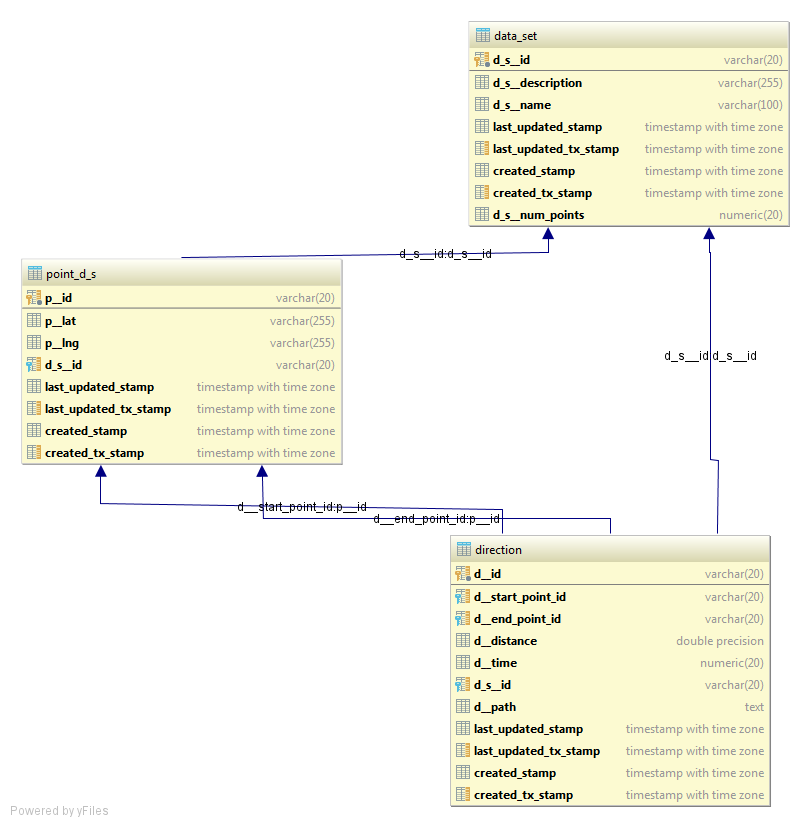
\includegraphics[scale=0.6]{database.png}
\caption{Thiết kế cơ sở dữ liệu của ứng dụng}
\label{database}
\end{figure}
\section{Các màn hình}
Ứng dựn được thiết kế gồm các màn hình sau: 
\begin{itemize}
\item[-] Màn hình tạo và sửa bộ dữ liệu (\ref{makedata}, \ref{editdata}).
\item[-] Màn hình lập lịch (\ref{laplich})
\item[-] Màn hình hiển thị kết quả (\ref{solution1}, \ref{solution2}).
\end{itemize}
\begin{figure}

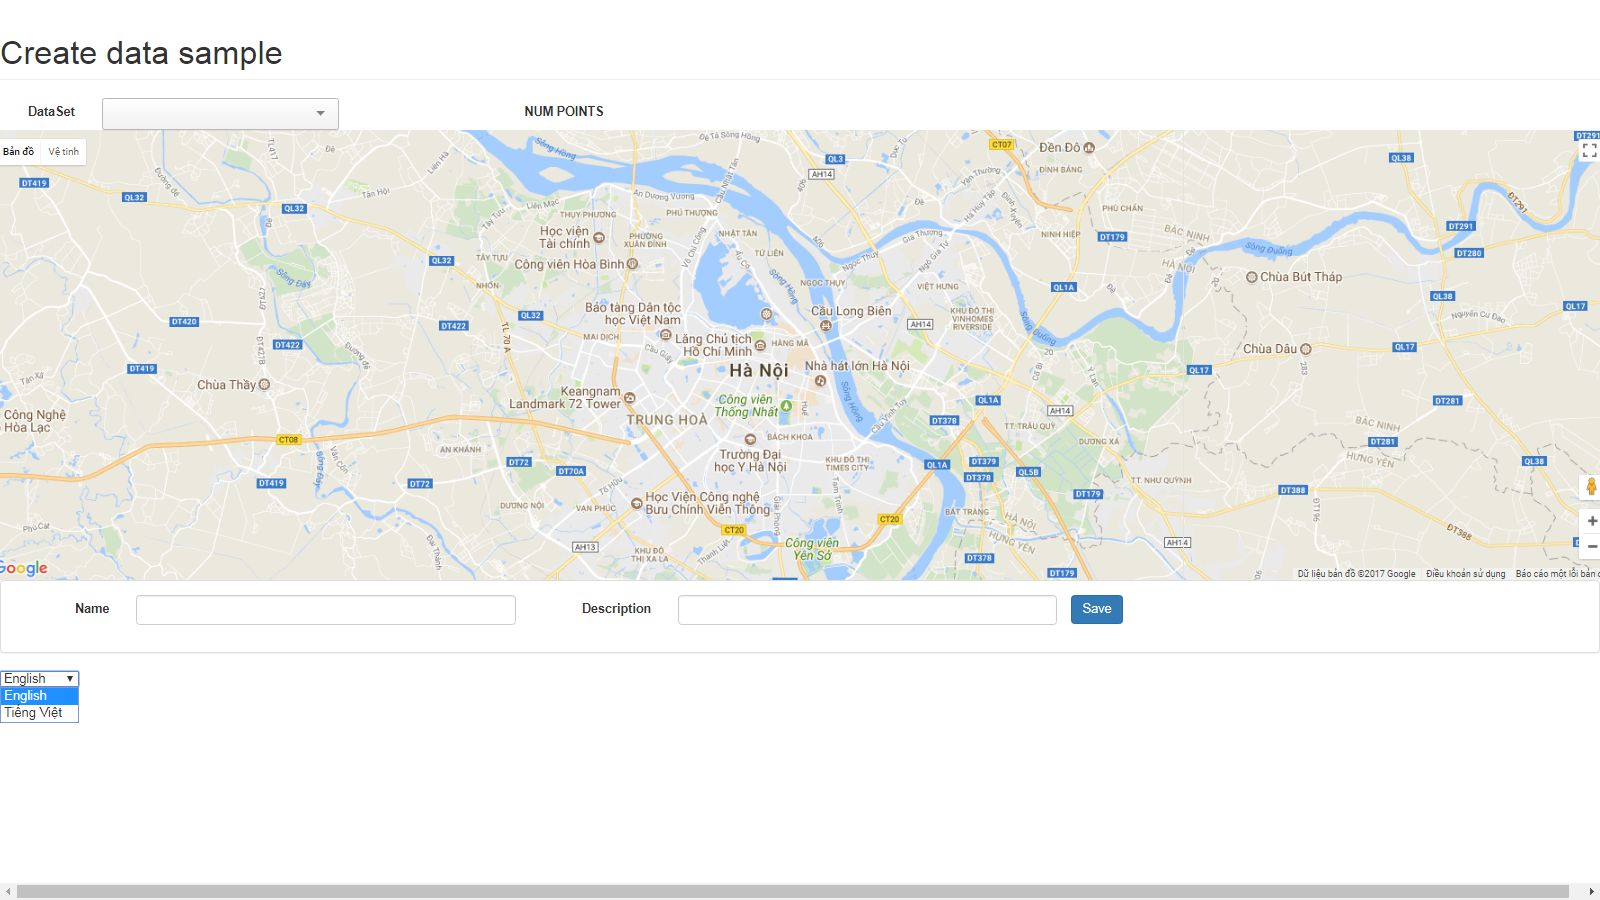
\includegraphics[scale=0.41]{screen/changeLanguage.png}
\caption{Màn hình thay đổi ngôn ngữ sang tiếng Anh}
\label{changelanguage}
\end{figure}

\begin{figure}

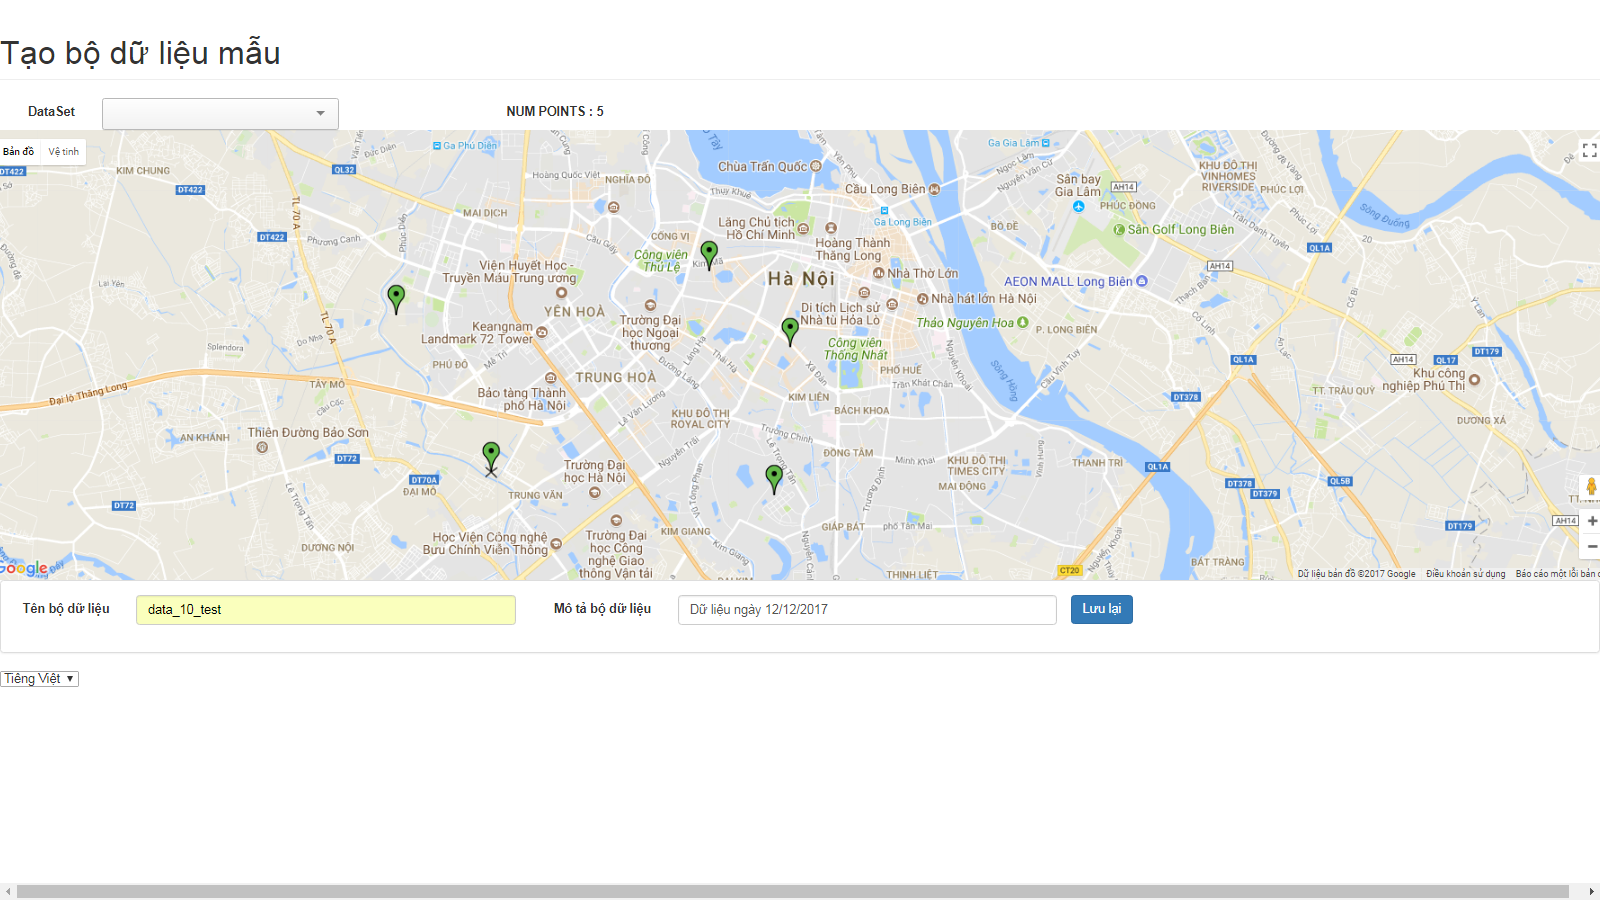
\includegraphics[scale=0.41]{screen/makedata.png}
\caption{Màn hình tạo dữ liệu lập lịch}
\label{makedata}
\end{figure}
\begin{figure}

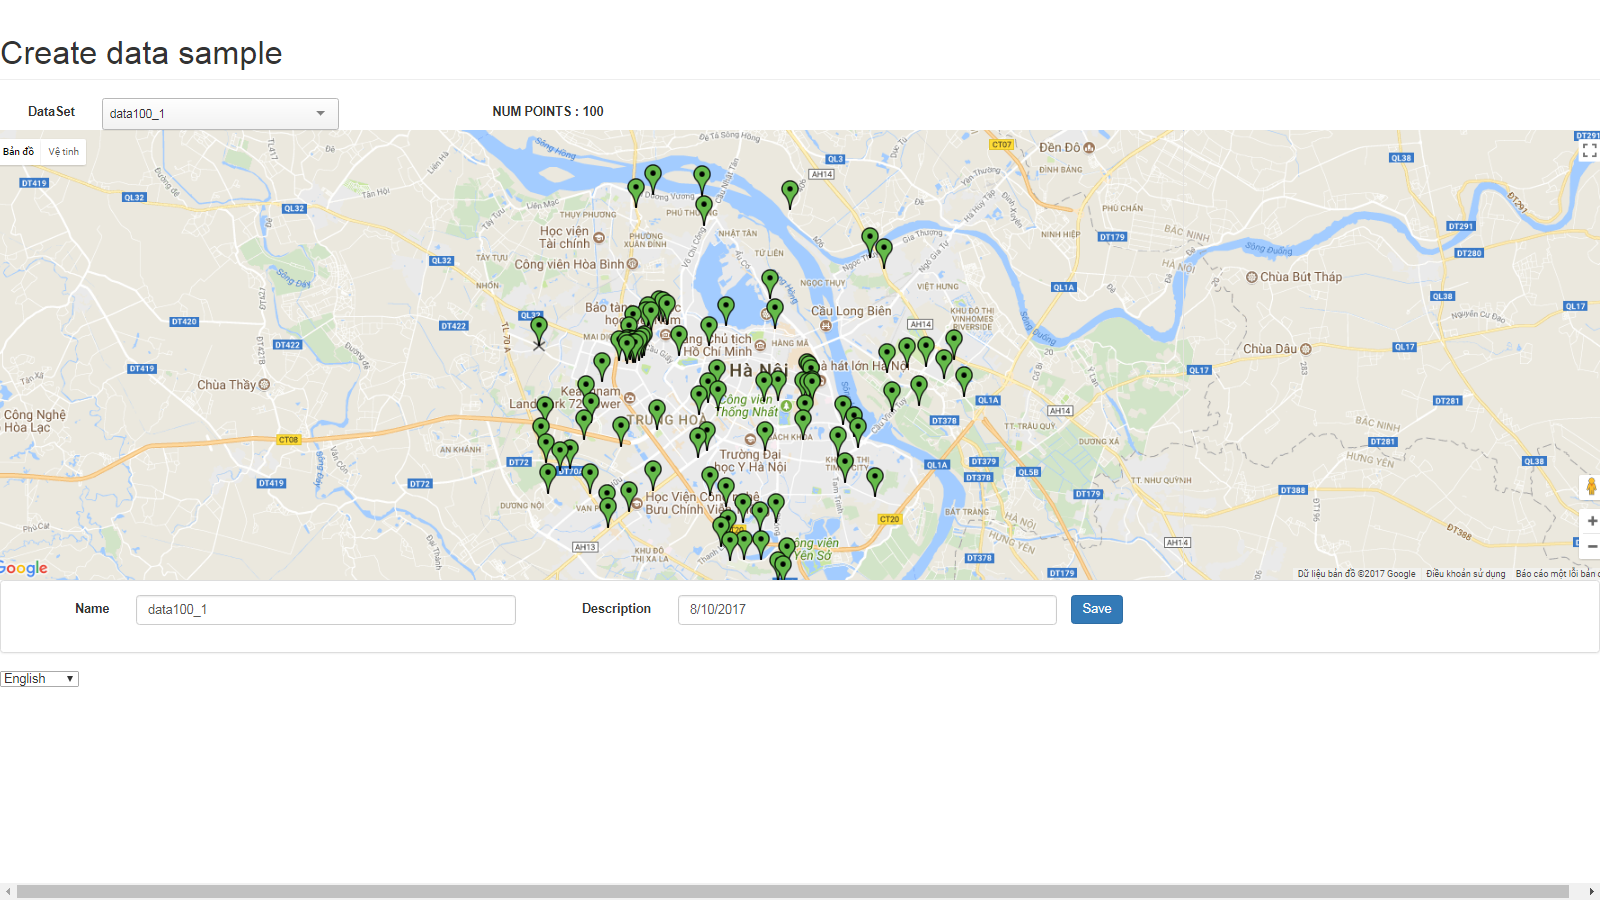
\includegraphics[scale=0.41]{screen/editdata.png}
\caption{Màn hình chỉnh sửa tập dữ liệu}
\label{editdata}
\end{figure}
\begin{figure}

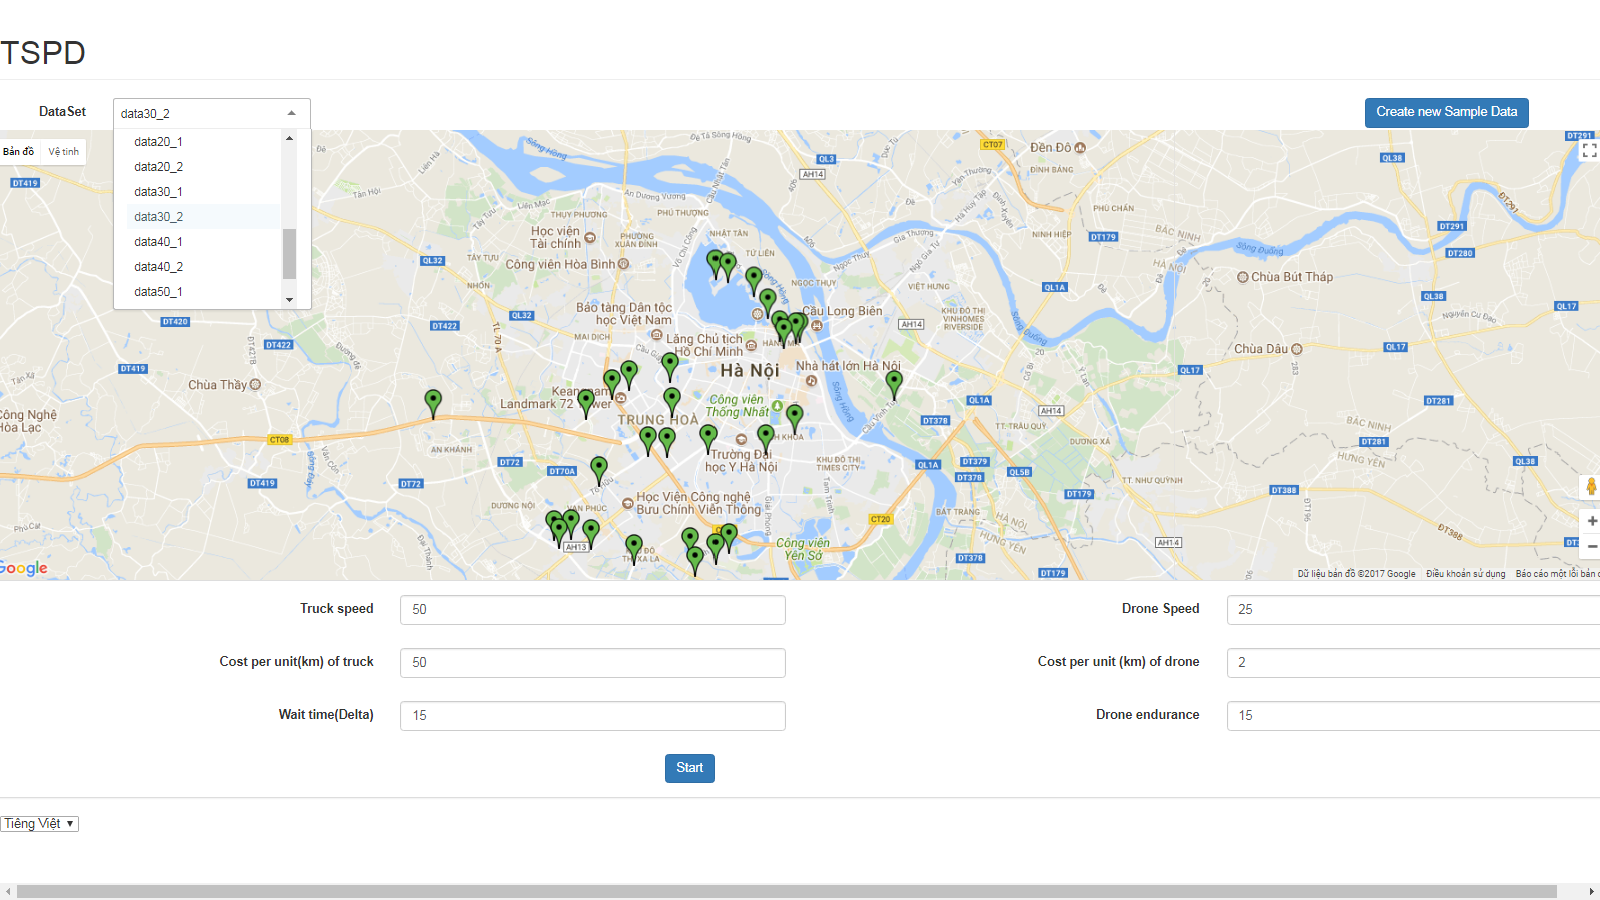
\includegraphics[scale=0.41]{screen/laplich.png}
\caption{Màn hình lập lịch}
\label{laplich}
\end{figure}
\begin{figure}

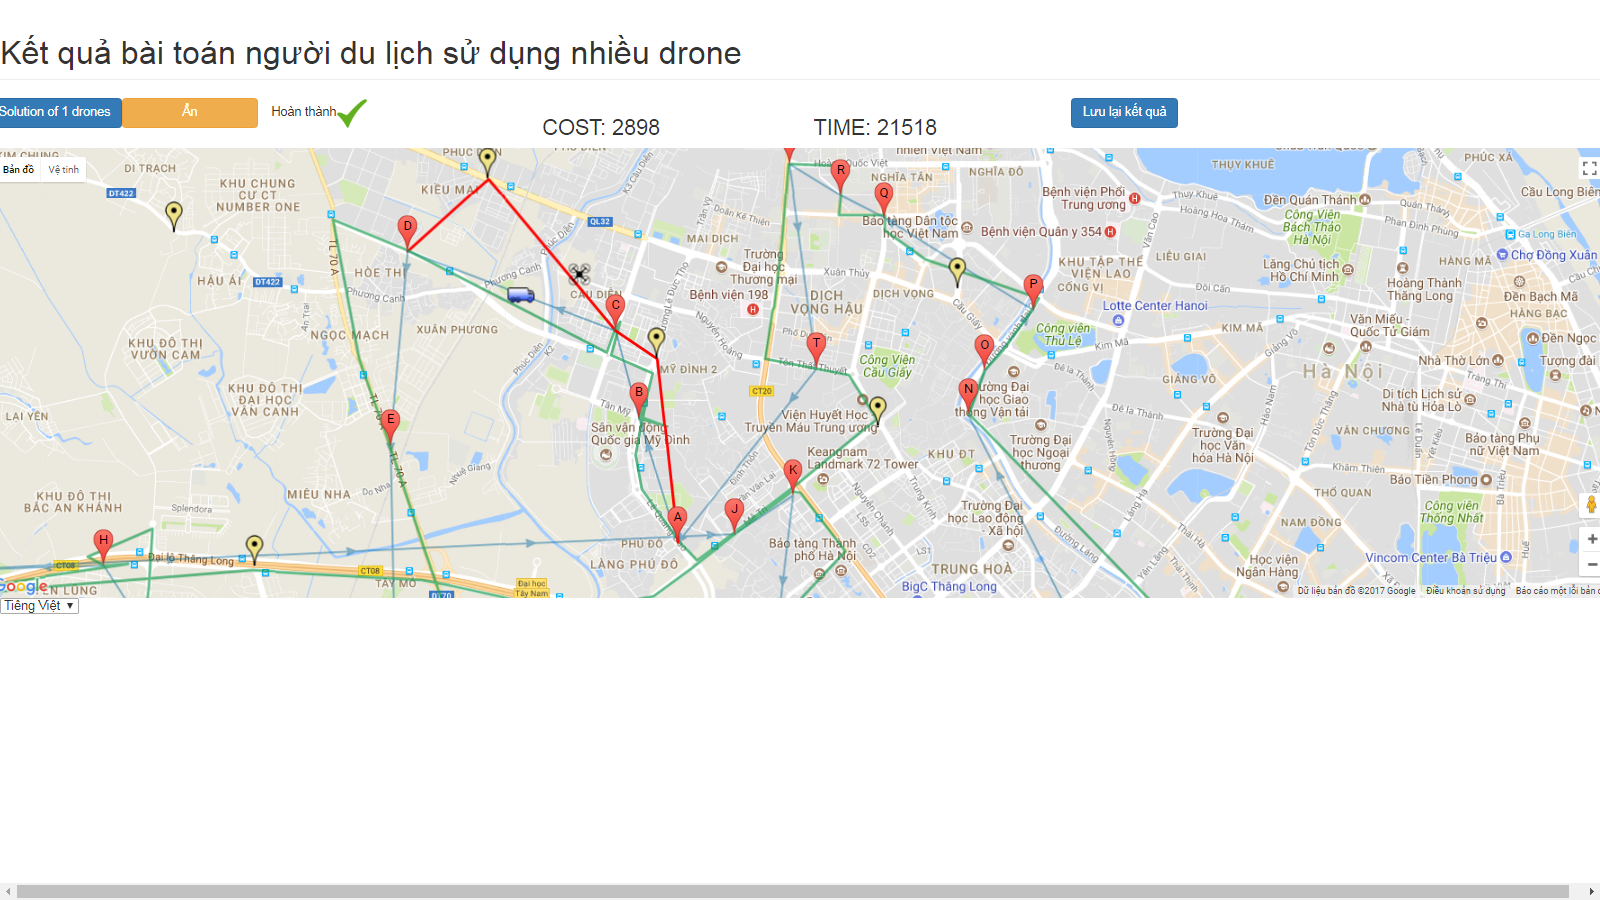
\includegraphics[scale=0.41]{screen/solution1.png}
\caption{Màn hình kết quả với một drone}
\label{solution1}
\end{figure}
\begin{figure}

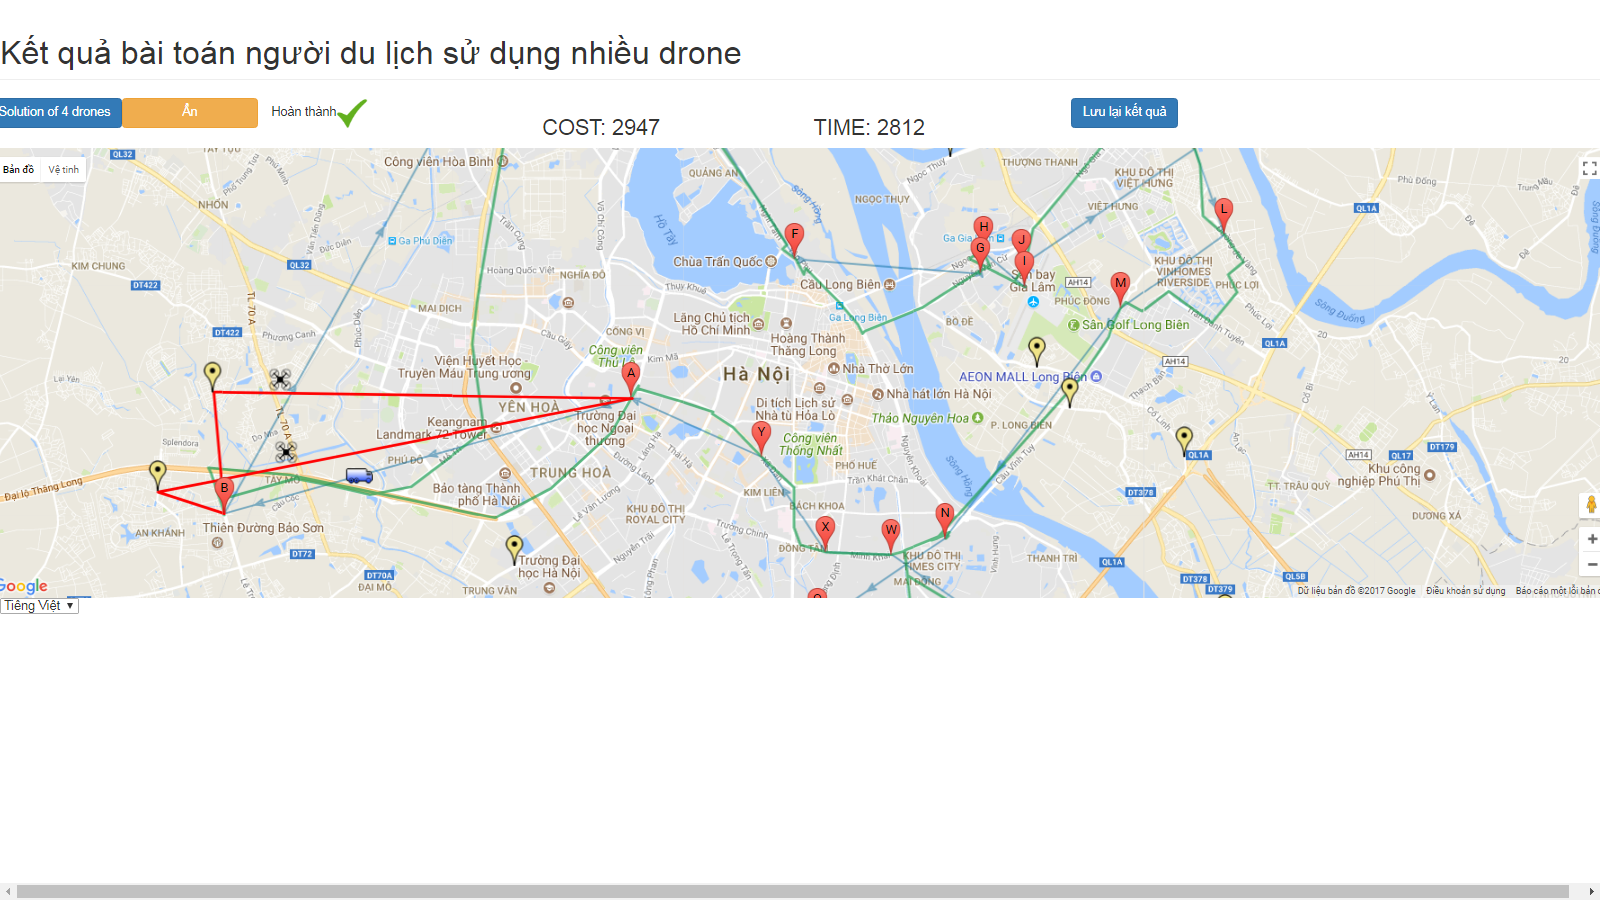
\includegraphics[scale=0.41]{screen/solution2.png}
\caption{Màn hình kết quả với bốn drone}
\label{solution2}
\end{figure}
\addcontentsline{toc}{chapter}{Kết luận và hướng phát triển}
\chapter*{Kết luận và hướng phát triển}
Lập kế hoạch vận tải hàng hoá là một lĩnh vực đặc biệt quan trọng trong nền kinh tế mỗi quốc gia. Các mô hình vận tải mới không ngừng được đề xuất mang lại thuận tiện, giảm chi phí vận tải. Trong đồ án này, chúng tôi khảo sát mô hình vận tải hang hoá kết hợp xe tải và thiết bị bay Drone. Xe tải có khả năng vận chuyển các hang hoá nặng, di chuyển trên hành trình dài, trong khi thiết bị bay Drone chỉ có khả năng vận chuyển hang hoá nhẹ, nhanh, nhưng quãng đường di chuyển ngắn do hạn chế về năng lượng nạp. 

Cụ thể, đồ án dựa trên nghiên cứu của Hà Quang Minh và cộng sự trong đó đề xuất thuật toán heuristics giải bài toán lập lộ trình vận tải kết hợp 1 xe tải và 1 thiết bị bay với mục tiêu là chi phí nhỏ nhất. Chúng tôi đã đề xuất thử nghiệm mô hình 1 xe tải kết hợp với nhiều thiết bị bay (2,3,4). Chúng tôi đã cài đặt thuật toán được đề xuất bởi Hà Quang Minh cho mô hình với nhiều Drone***. Kết quả thử nghiệm cho thấy bằng việc kết hợp với nhiều hơn 1 drone thì chi phí sẽ giảm hơn so với việc sử dung 1 drone.

Trong tương lai, chúng tôi sẽ cố gắng phát triển thuật toán trên các mô hình vận chuyển hàng hóa kết hợp xe tải và drone khác như: bài toán vận chuyển hàng hóa kết hợp xe tải và drone nhiều lộ trình, bài toán nhận hàng và đón hàng kết hợp xe tải và drone \ldots. Ngoài ra chúng tôi cũng thiết kế và cài đặt thêm một vài thuật toán với heuristic mới để đem lại kết quả tốt hơn nữa cho bài toán.

\begin{thebibliography}{9}
\bibitem{csplib30} \url{http://www.csplib.org/Problems/prob030/}
\bibitem{slidethayquang} Slide Trí tuệ nhân tạo thầy Nguyễn Nhật Quang. Chương 5 : Thỏa mãn ràng buộc
\bibitem{AIAMAB} Stuart Russell and Peter Norvig 
\textit{Artificial Intelligence: A Modern Approach} 2\textsuperscript{nd } edition, Prentice Hall, page 137,  2003.
\bibitem{main} Ha Quang Minh and Deville Yves and Pham Quang Dung and Ha Minh Hoang, \textit{On the min cost traveling salesman problem with drone}, arXiv preprint arXiv:1509.08764, 2015
\bibitem{bahiwww} S. Banker, Amazon and drones – here is why it will work (dec 2013).
URL \url{http://www.forbes.com/sites/stevebanker/2013/12/19/amazon-drones-here-is-why-it-will-work/}
\bibitem{TRR} Nguyễn Đức Nghĩa, Nguyễn Tô Thành 
\textit{Toán rời rạc} 3\textsuperscript{rd} edition, Nhà xuất bản đại học quốc gia Hà Nội, page 107-108,  2006.
\bibitem{TUHTT} Slide Tối ưu hóa tổ hợp thầy Nguyễn Đức Nghĩa. Chương mở đầu, Bài toán vận tải.
\bibitem{CBLS} Slide Tìm kiếm cục bộ dựa trên ràng buộc thầy Phạm Quang Dũng. Chương 5: Contraint-base local search applications.
\bibitem{DAA} Slide Phân tích và thiết kế thuật toán thầy Nguyễn Đức Nghĩa. Chương 5: Quy hoạch động, Chương 3: Greedy Algorithms.
\bibitem{HCP} Francesca Rossi, Peter van Beek, Toby Walsh 
\textit{Handbook of Constraint Programming} 1\textsuperscript{st} edition, Elsevier Science, page 107-108,  2006.
\bibitem{GA} Bài giảng môn tính toán tiến hóa cô Huỳnh Thị Thanh Bình. Thuật giải di truyền.
\bibitem{AODTBT}Rupert Howell,Jonathon Wong
\textit{Apache OFBiz Development: The Beginner's Tutorial}, Paperback , page 53,  2008.
truyền.
\bibitem{AOC} Ruth Hoffman
\textit{Apache OFBiz Cookbook}, Paperback , page 28, 2010.
\bibitem{AOW} Apache Ofbiz (wikipedia)
\url{https://en.wikipedia.org/wiki/Apache_OFBiz}
\end{thebibliography}


\end{document}
